\chapter{Implementation}\label{cha:implementation}

A number of components were created to implement the proposed architecture. This chapter will provide a high-level overview of the solution, then examine each component in further detail.

\section{Overall Solution}
\begin{figure}[h]
	\centering
	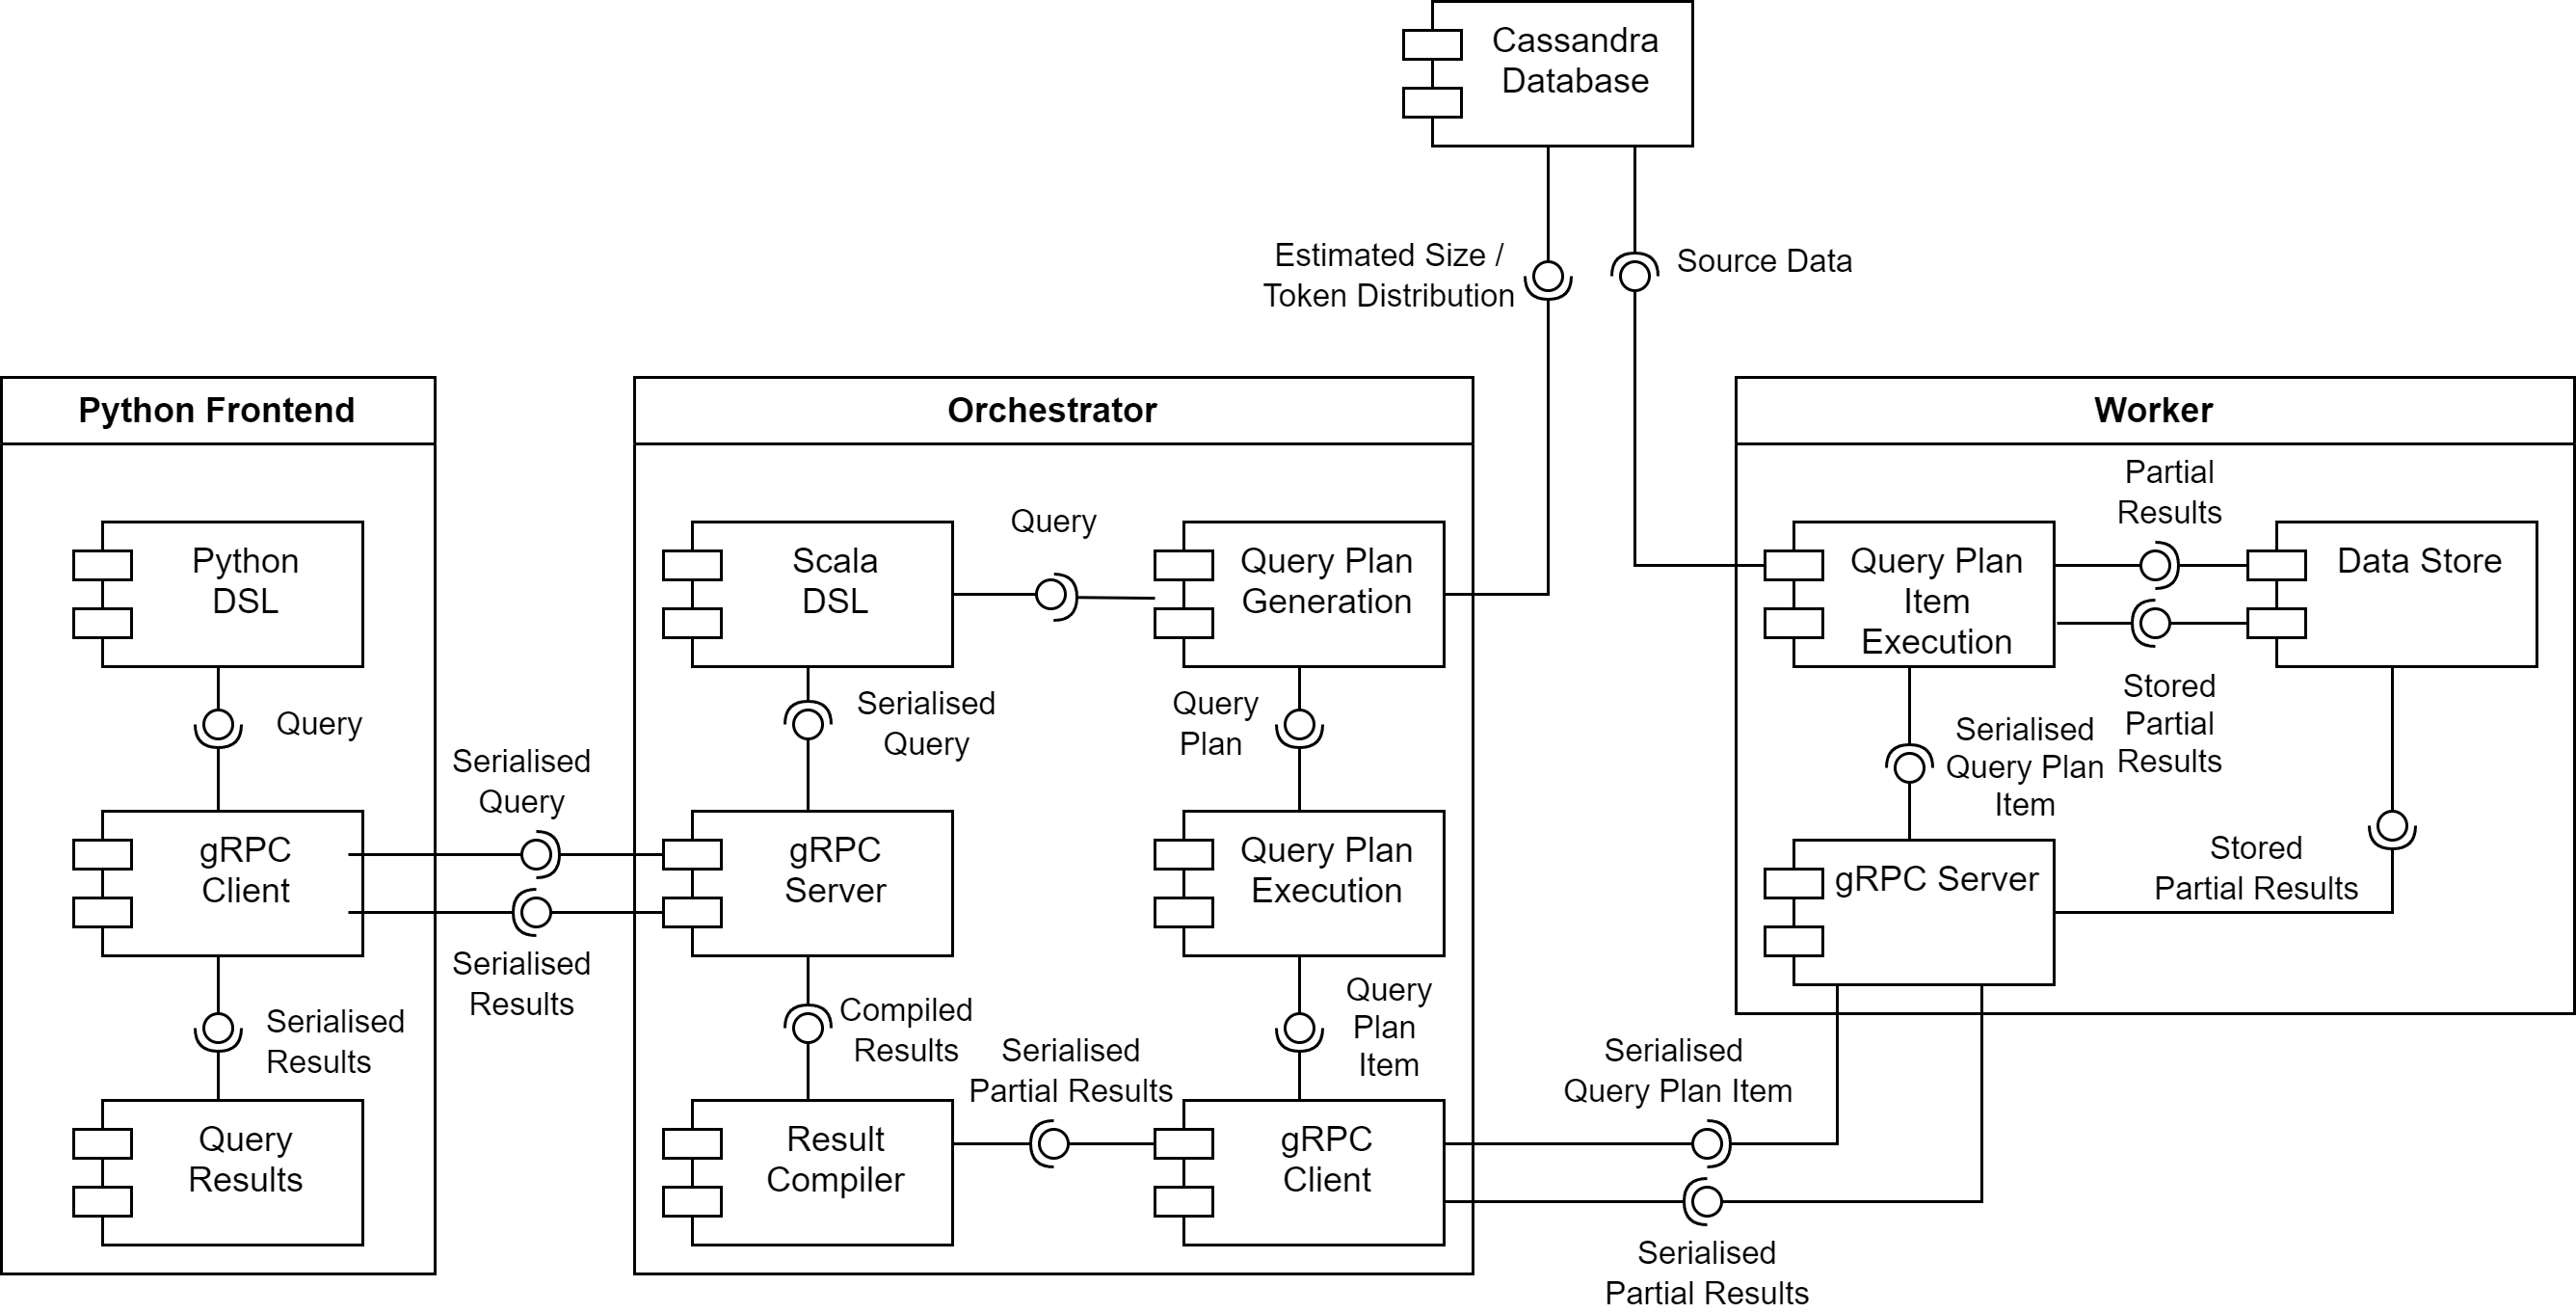
\includegraphics[width=0.7\textwidth]{chapters/diagrams/implementation/component-architecture-diagram}
	\caption{Solution Component Diagram}
	\label{fig:component-architecture-diagram}
\end{figure}

Figure \ref{fig:component-architecture-diagram} is a component diagram describing the interactions of the core components. As described in Section \ref{sec:architecture}, the user accesses the system through the frontend. This is a terminal, allowing the user to define queries using the Python Domain Specific Language (DSL), and receive results. Queries are sent to the orchestrator, which controls the state of the system. To execute a query, it generates a query plan which describes the steps for computing a result. Then, the query plan is executed step-by-step, with the data used in each step being split up into chunks of work (partitions) before being delegated to the workers, which are responsible for actually computing partitions. When all query plan steps have been executed, the orchestrator collates the partial results from all workers, and returns the final result to the frontend. gRPC is used for network communication between the frontend, orchestrator and worker nodes.

The system supports three query types: Select, Filter and Group By. Select and Filter are row-level operations, meaning the workers do not have to share data during computation. However, Group By does need the workers to cross-communicate, so a temporary store is needed to cache partial results.

\section{Type System}\label{sec:type-system}
The type system's role is to provide a representation for every type of value the user can store within a table. However, designing the interfaces to represent these values presents a challenge. Figure \ref{fig:type-system-motivation} demonstrates the problem. 

On the left, an example is shown where a table is a 2D list of raw values. As multiple types are stored in the same list, there is no shared type information between the values, so they cannot be used to determine the table's contents. To discover a value's type, the system would have to perform runtime type checks against all supported types, adding a significant amount of overhead. 

On the right, a conceptual model using a container class is shown. The container stores a raw value with the type information about the value, and the table is a 2D list of containers. The system only needs to perform one runtime type check in order to instantiate the correct container instance. 

\begin{figure}[htp]
	\centering
	% left - data stored in raw format - no information 
	% right - data stored in containers with value and type information, can infer what type the value is from the stored type information
	\centering
	\subfloat[\centering Raw Data - No Type Information Available]{
		\begin{tabular}{r c c l}
			\textbf{Header:} [& id, & name & ] \\
			\textbf{Row 1:} [& 1, & "Alice" & ] \\
			\textbf{Row 2:} [& 2, & "Bob" & ] \\
		\end{tabular}
	}
	\qquad
	\subfloat[\centering Container Class - Value and Type Information Stored Together]{
		\begin{tabular}{r c c l}
			\textbf{Header:} [& (id, int), & (name, string) & ] \\
			\textbf{Row 1:} [& (1, int), & ("Alice", string) & ] \\
			\textbf{Row 2:} [& (2, int), & ("Bob", string) & ] \\
		\end{tabular}
	}
	\caption{Type System - Motivating Example}
	\label{fig:type-system-motivation}
\end{figure}

Due to Java limitations, this conceptual solution is not straightforward to implement. The container class could use a generic type parameter which stores the type information of the value, but generic type information is erased at runtime \cite{ghosh2004generics}. Instead, it could be defined as an interface, with subclass implementations for each supported type, but this is not much better than the raw data solution, as the runtime type check simply becomes a pattern match on the class type. A solution that exploits some kind of polymorphism is preferred. 

Scala provides a feature known as \textit{ClassTags} \cite{scalaclasstags}. These save the erased type information and support equality checks between \textit{ClassTag} instances, meaning the framework can use them to compare the type of a value to an expected type. The conceptual container class is therefore defined as an interface \textit{ValueType}, which holds a \textit{ClassTag} instance. This interface is implemented by \textit{TableField}, which holds a field name and its type, and \textit{TableValue}, which holds a value and its type. Concrete implementations for the 5 supported types described in Section \ref{subsec:supported-types} are provided for both subclasses. Figure \ref{fig:type-system-hierarchy} shows the class hierarchy.

\begin{figure}[htp]
	\centering
	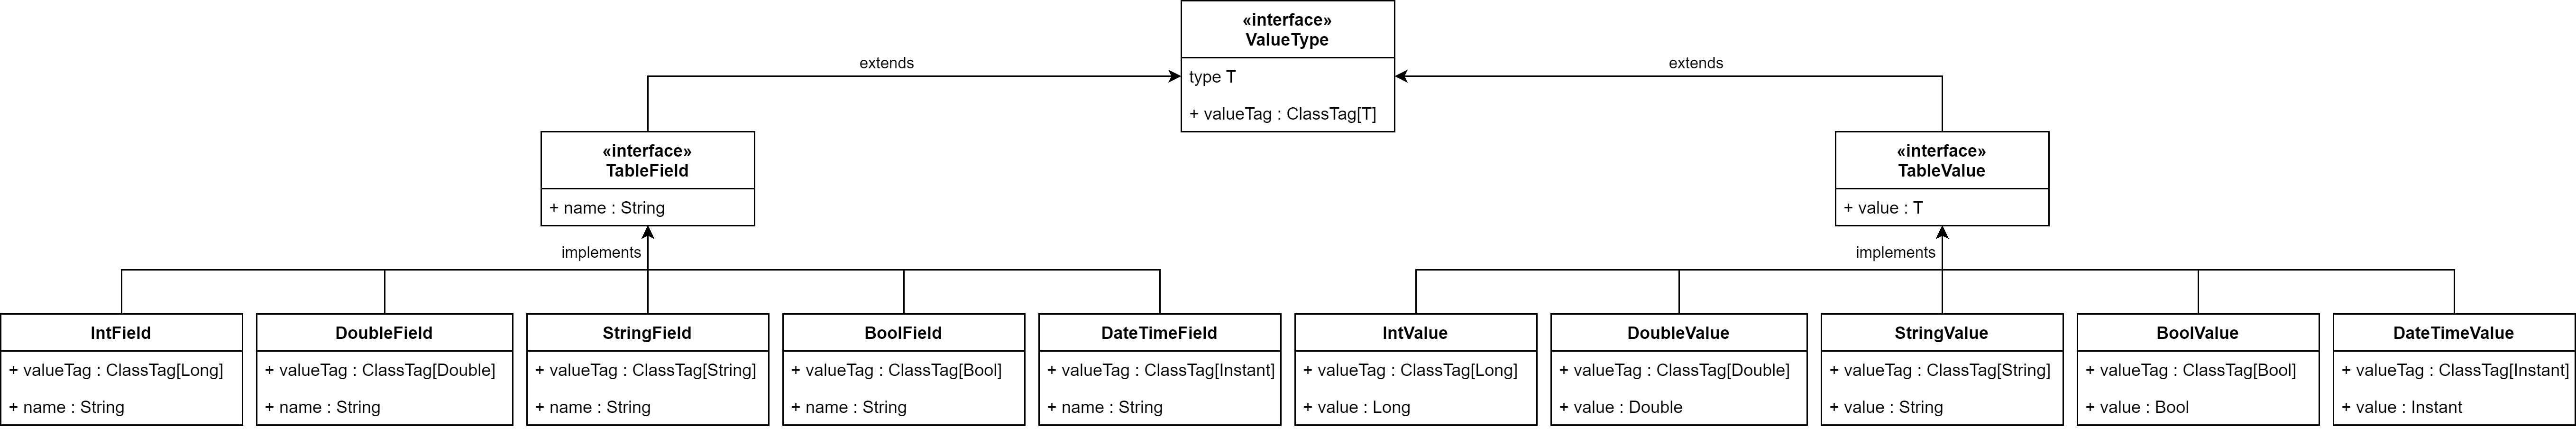
\includegraphics[width=0.7\textwidth]{chapters/diagrams/implementation/type-system-hierarchy}
	\caption{Custom Type System Hierarchy}
	\label{fig:type-system-hierarchy}
\end{figure}

\pagebreak
\subsection{Supported Types}\label{subsec:supported-types}
The type system supports a subset of Scala, Python, and Cassandra's types, shown in Figure \ref{fig:datatypes}. These types were selected to ensure they could be represented in all parts of the system, including when serialising to protobuf format.

\begin{figure}[htp]
	\centering
	\begin{tabular}{| c | c | c | c |}
		\hline
		\textbf{Base Type} & \textbf{Python} & \textbf{Scala} & \textbf{Cassandra} \\ \hline
		Integer & int & Long & bigint \\ \hline
		Float & float & Double & double \\ \hline
		String & string & String & text \\ \hline
		Boolean & boolean & Boolean & boolean \\ \hline
		DateTime & datetime & Instant & timestamp \\ \hline
	\end{tabular}
	\caption{Primitive Types}
	\label{fig:datatypes}
\end{figure}

\subsection{Result Model}
The hierarchy of classes and supported types provide everything needed to define a table of result data, known as a \textit{TableResult}. Headers are a sequence of \textit{TableFields} and result rows are a two-dimensional array of \texttt{Option[TableValue]}. As defined in the requirements, null values must be supported, but this is discouraged in Scala. Instead, Option is preferred as it is supported by all the typical functional methods. In this model, values are represented by \texttt{Some(TableValue())}, and null values are represented by \texttt{None}. Figure \ref{fig:example-table-result} shows an example \textit{TableResult}.

\begin{figure}[htp]
	\centering
	\begin{tabular}{l c  c  c l}
		\textbf{Header:} [ & IntField(\textcolor{deepgreen}{"ID"}),  & StringField(\textcolor{deepgreen}{"Name"}),  & BoolField(\textcolor{deepgreen}{"Passed"}) & ] \\
		\textbf{Row 1:} [[ & Some(IntValue(1)), & Some(StringValue(\textcolor{deepgreen}{"Alice"})), & Some(BoolValue(true)) & ], \\
		\textbf{Row 2:}  [ & Some(IntValue(2)), & None, & None & ], \\
		\textbf{Row 3:}  [ & Some(IntValue(3)), & Some(StringValue(\textcolor{deepgreen}{"Bob"})), & None & ]] \\
	\end{tabular}
	\caption{\textit{TableResult} example}
	\label{fig:example-table-result}
\end{figure}

\pagebreak
\section{Domain Specific Language}
The user interacts with the framework through the Domain Specific Language (DSL), which is modelled with SQL-like syntax. Users can define expressions, then use these in computations like Select, Filter and Group By. Figure \ref{fig:dsl-high-level-example} shows an annotated DSL query, with links to the sections where each part is discussed further.

\begin{figure}[htp]
	Initialise cluster connection and select a Cassandra source table (Section \ref{subsec:cassandra}):
	\begin{python}
ClusterManager("orchestrator-url")
  .cassandra_table("example", "table")
	\end{python}
	
	Select (Section \ref{subsec:select-computation}), uses \textit{FieldExpressions} (Section \ref{subsec:fieldexpressions}) and Python Operators (Section \ref{subsec:dsl-python}):
	\begin{python}
  .select(
    F("id"),
    (F("duration") * 2).as_name("duration2"),
    Function.Left(Function.ToString(F("date")), 8)
      .as_name("yyyy-mm")
  )
	\end{python}

	Filter (Section \ref{subsec:filter-computation}), uses \textit{FieldComparisons} (Section \ref{subsec:fieldcomparisons}) and Python Operators (Section \ref{subsec:dsl-python}):
	\begin{python}
  .filter(
    (F("duration2") > 40) && 
  	(F("yyyy-mm").contains("2021")
  )
	\end{python}

	Group By (Section \ref{subsec:group-by}), uses \textit{AggregateExpressions} (Section \ref{subsec:aggregateexpressions}):
	\begin{python}
  .group_by(
    [F("duration2")],
    [
      Max(F("id")),
      Count(F("yyyy-mm"))
    ]
  )
	\end{python}
	\caption{Example DSL Query}
	\label{fig:dsl-high-level-example}
\end{figure}

\pagebreak
\subsection{FieldExpressions}\label{subsec:fieldexpressions}
\textit{FieldExpressions} allow the user to define arbitrary row-level calculations. They are defined as an interface, with three subclasses:

\begin{itemize}
	\item Values: define literal values which never change across all rows.
	\item Fields: get the value at the current row for the given field name.
	\item FunctionCalls: perform arbitrary function calls using \textit{FieldExpressions} as arguments.
\end{itemize}

Figure \ref{fig:field-expressions-examples} provides examples for each type of \textit{FieldExpression}.

\begin{figure}[htp]
	Values (from left to right): string \texttt{"a"}, integer \texttt{1}, double \texttt{1.5}, boolean \texttt{True}, date \texttt{31/12/2021}.
	\begin{python}
V("a") , V(1), V(1.5), V(True), V(datetime.date(2021, 12, 31))
	\end{python}

	Fields (from left to right): \texttt{fieldName}, \texttt{duration}, \texttt{id}, \texttt{creationDate}.
	\begin{python}
F("fieldName"), F("duration"), F("id"), F("creationDate")
	\end{python}

	Top Function: convert \texttt{field1} to a string, then take the left 10 characters of each row.
	
	Bottom Function: multiply \texttt{field2} by 2, then divide by \texttt{field3}
	\begin{python}
Function.Left(Function.ToString(F("field1")), 10)
(F("field2") * 2) / F("field3")
	\end{python}
	\caption{\textit{FieldExpression} implementations and examples}
	\label{fig:field-expressions-examples}
\end{figure}

Many basic functions have been implemented, including arithmetic, string and cast operations. However, the function system is designed to be extensible. A number of helper classes and interfaces are provided to do this, with the main constraint being that functions can only take the 5 primitive types as arguments.

\paragraph{Type Resolution} 
Type Resolution is performed in two stages: resolution, and evaluation. The resolution step takes in type information from the input result header, and verifies that the \textit{FieldExpression} is well-typed with regards to that result by comparing \textit{ClassTags}; see Section \ref{sec:type-system} for details. The evaluation step performs the computation on a \textit{TableResult} row without any type checking. Unchecked casts are used here instead, demonstrated for a binary function in Figure \ref{fig:fieldexpression-unchecked-casts}. 

\begin{figure}[htp]
	\centering
	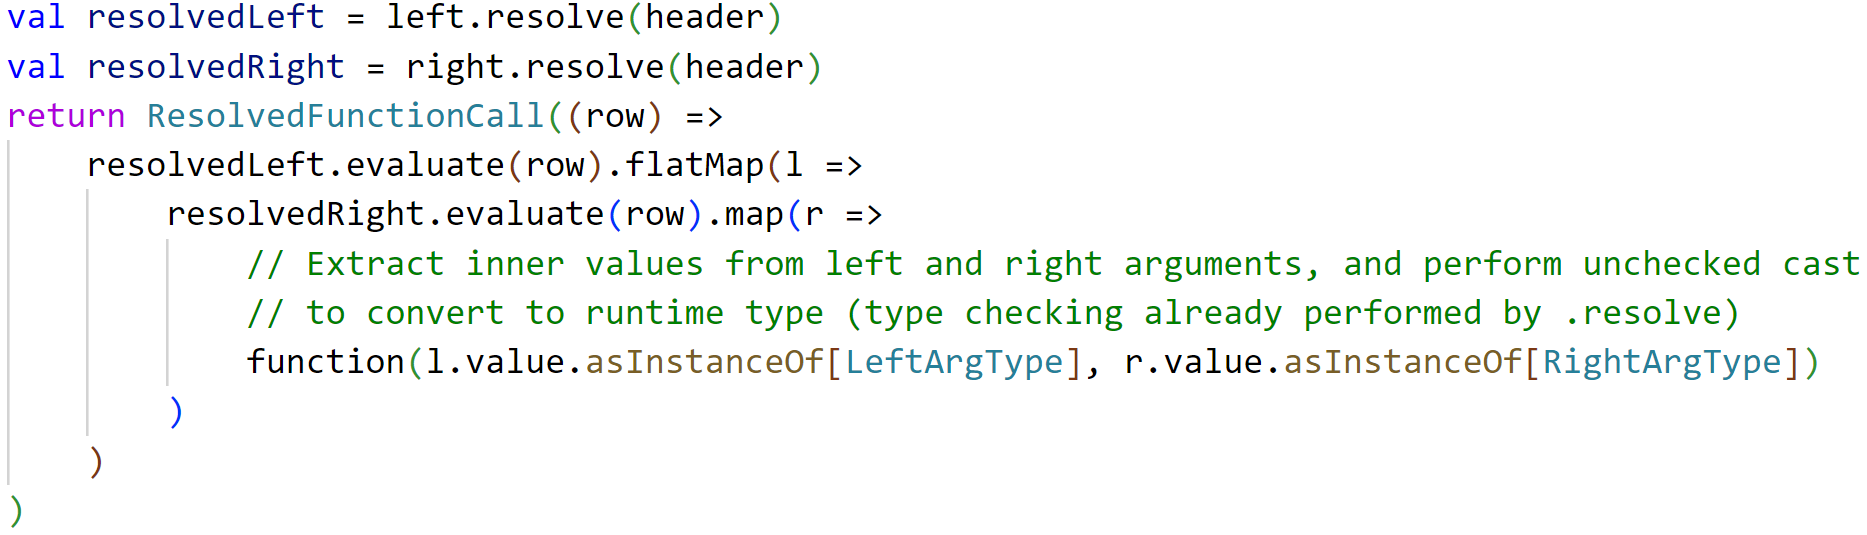
\includegraphics[width=\textwidth]{chapters/diagrams/implementation/type-resolution-unchecked-casts}
	\caption{Runtime Evaluation of Functions}
	\label{fig:fieldexpression-unchecked-casts}
\end{figure}

\pagebreak
The resolution step catches two key types of invalid expression. Firstly, a Field reference is invalid if the field name is not present in the table header, shown in Figure \ref{fig:field-type-resolution}. Secondly, a Function call is invalid if an argument returns an invalid type, shown in Figure \ref{fig:function-type-resolution}.

\begin{figure}[htp]
	\centering
	For the expression F(\textcolor{deepgreen}{"field"}):
	
	\subfloat[\centering Valid - \textcolor{deepgreen}{"field"} is present in the header]{
		\begin{tabular}{l c l}
			\textbf{Header:} [& IntField(\textcolor{deepgreen}{"field"}) ] \\
		\end{tabular}
	}
	\qquad
	\subfloat[\centering Invalid - \textcolor{deepgreen}{"field"} not present in the header]{
		\begin{tabular}{l c l}
			\textbf{Header:} [& StringField(\textcolor{deepgreen}{"differentField"}) ] \\
		\end{tabular}
	}
	\caption{Type Resolution of Fields}
	\label{fig:field-type-resolution}
\end{figure}

\begin{figure}[h]
	Valid - both arguments to \textit{Concat} are strings:
	\begin{python}
Function.Concat(V("hello"), V("Alice"))
	\end{python}
	
	Invalid - \textit{V(1)} is not a string:
	\begin{python}
Function.Concat(V("hello"), V(1))
	\end{python}
	\caption{Type Resolution of Functions}
	\label{fig:function-type-resolution}
\end{figure}

A two-step process has a number of benefits. The resolution step enables a form of polymorphism on some functions like arithmetic operations. These determine what types are returned by their sub-expressions during resolution, and change their behaviour for evaluation. For example, the add function resolves to \textit{AddInt}, \textit{AddDouble}, or \textit{Concat}. It also reduces the overhead at runtime as type checking does not need to be performed for each row.

\paragraph{Named Expressions}
When performing a Select operation, the output fields must be named to so operations can reference fields from the previous input. Figure \ref{fig:namedfieldexpression-examples} shows the two ways of naming a field: \textit{FieldExpressions} can be assigned a name, and single Field references will keep their previous name.

\begin{figure}[htp]
	Top Expression Name: \texttt{twice\textunderscore duration}
	
	Bottom Expression Name: \texttt{creation\textunderscore date}
	\begin{python}
(F("duration") * 2).as_name("twice_duration")
F("creation_date")
	\end{python}
	\caption{\textit{NamedFieldExpression} examples}
	\label{fig:namedfieldexpression-examples}
\end{figure}

\pagebreak
\subsection{FieldComparisons}\label{subsec:fieldcomparisons}
\textit{FieldComparisons} allow the user to define arbitrary row-level comparisons. They are defined as an interface, supporting a number of comparison types including null, equality, numerical and string comparisons. Examples of each are shown in Figure \ref{fig:field-comparisons-examples}.

\begin{figure}[htp]
	Null checks: verify whether an expression is null or not null.
	\begin{python}
F("duration").is_null()
F("duration").is_not_null()
	\end{python}
	
	Equality checks: verify whether two \textit{FieldExpressions} are equal or not equal. 
	\begin{python}
F("duration") == 20
F("duration") != F("other_duration")
	\end{python}

	Ordering checks: apply ordered comparators between two \textit{FieldExpressions}.
	\begin{python}
F("duration") < 20
F("duration") <= 19
F("duration") > 20
F("duration") >= 21
	\end{python}

	String checks: apply contains, starts with and ends with operators (case insensitive versions also available).
	\begin{python}
F("name").contains("Alice")
F("name").starts_with("Bob")
F("name").ends_with("Smith")
	\end{python}
	\caption{\textit{FieldComparison} examples}
	\label{fig:field-comparisons-examples}
\end{figure}

\paragraph{Combined Comparisons}
The user can combine multiple \textit{FieldComparisons} using AND/OR operators, shown in Figure \ref{fig:field-comparisons-combiners}. This is implemented around Scala's own boolean operators, meaning optimisations like short circuiting operate as normal.

\begin{figure}[htp]
	\begin{python}
(F("duration") < 20) && (F("name").starts_with("Bob"))
(F("duration") < 20) || (F("name").starts_with("Bob"))
(F("duration") < 20) && (
  (F("name").contains("Bob")) || (F("name").contains("Alice"))
)
	\end{python}
	\caption{\textit{FieldComparison} AND/OR Combinations}
	\label{fig:field-comparisons-combiners}
\end{figure}

\pagebreak
\subsection{Aggregate Expressions}\label{subsec:aggregateexpressions}
\textit{AggregateExpressions} are only used in Group Bys, taking a \textit{NamedFieldExpression} as an argument, and aggregating any number of input result rows into a single result using \textit{reduce}. Figure \ref{fig:aggregate-expressions-all} demonstrates all supported operations.

%The supported operations are Minimum, Maximum, Sum, Average, Count, and String Concatenation, and they are polymorphic where possible. For example, minimum and maximum handle numeric types by ordering numerically and string types lexicographically. Figure \ref{fig:aggregate-expressions-examples} shows examples of \textit{AggregateExpressions}.

\begin{figure}[htp]
	Minimum/Maximum - supports integers, floats and dates (ordered numerically), strings (ordered lexicographically):
	\begin{python}
Min(F("duration"))
Max(Function.ToString(F("date")).as_name("date_string"))
	\end{python}

	Sum - supports integers and floats:
	\begin{python}
Sum(F("amount"))
	\end{python}
	
	Average - supports integers, floats and dates:
	\begin{python}
Avg(F("date"))
	\end{python}

	Count (and distinct) - supports all data types:
\begin{python}
Count(F("id"))
DistinctCount(F("date"))
\end{python}

	String Concatenation (and distinct) - combines all strings in a field with a given string delimiter.
\begin{python}
StringConcat(F("name"), ", ")
DistinctStringConcat(F("address"), ", ")
\end{python}
	\caption{\textit{AggregateExpression} examples}
	\label{fig:aggregate-expressions-all}
\end{figure}

\subsection{Protocol Buffer Serialisation}
Any DSL query can be serialised to protobuf format, allowing it to be sent using gRPC. \textit{TableResults} are also serialisable, to allow the system to return query results to the user. gRPC has a size limit of 4MB for individual messages, so \textit{TableResults} are streamed row-by-row.

\subsection{Python Implementation}\label{subsec:dsl-python}
The Python frontend is designed to be straightforward to use, hiding the complexities of the computation being performed in the backend. A number of Python-specific features were used to help with this.

Python allows developers to override common operators with custom definitions. The Python implementation of \textit{FieldExpression} overrides the arithmetic operators, as well as comparison operators to allow the user to automatically generate functions and \textit{FieldComparisons}, without having to write the full definition. % example?

Furthermore, as discussed in \ref{subsec:frontend-design}, pandas is widely used for Python data analysis \cite{reback2020pandas}. The frontend is able to convert query results from protobuf to a pandas DataFrame to aid further analysis.


\pagebreak
\section{Data Model}\label{subsec:data-model}
% This section should be clear and understandable, as much of the rest refers to partial and full versions
The data model is split into two key components: \textit{DataSource} and \textit{Table}. 

\textit{DataSource} is an interface, representing any part of the query where data must be rearranged into new partitions including Cassandra source data, and Group By operations. \textit{Table} is a class, representing the computation of any row-level operations like Select and Filter, which must implement the \textit{TableTransformation} interface. It is composed of a \textit{DataSource} and a list of \textit{TableTransformations}. To compute its output, the \textit{DataSource} is computed first, then all transformations are applied sequentially.

Optionally, \textit{DataSources} can have dependent \textit{Tables} which must be calculated first. For example, a Group By \textit{DataSource} requires a single \textit{Table} to be computed before it can be generated. A Cassandra \textit{DataSource} will always act as the terminal component for a query, as it has no dependencies.

Figure \ref{fig:filter-select-query} shows a Filter and Select query in the DSL, and the data model. Note that any number of Select and Filter operations can be added to the output table, as these operations do not require generating new partitions.

\begin{figure}[htp]
	\centering
	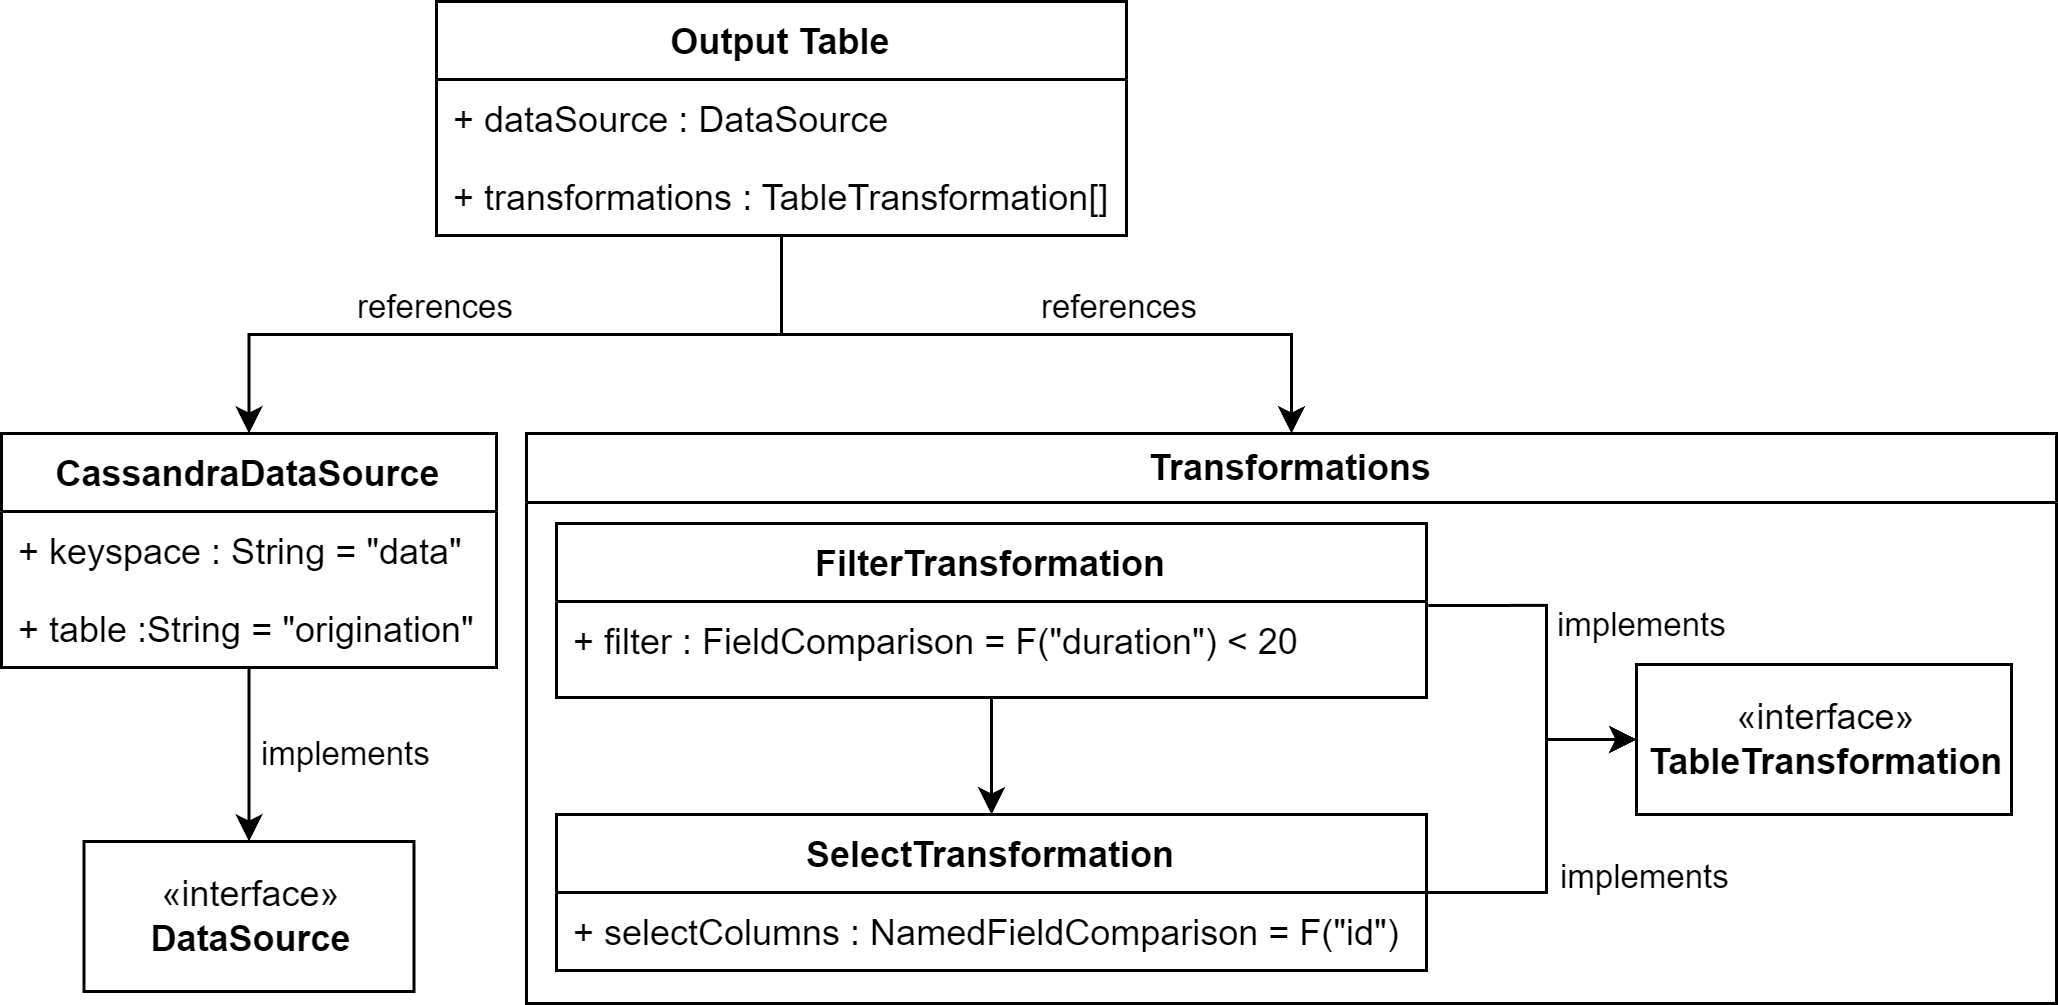
\includegraphics[width=0.8\textwidth]{chapters/diagrams/implementation/filter-select-query}
	\begin{python}
ClusterManager("orchestrator-service")
.cassandra_table("data", "origination")
.filter(F("duration") < 20)
.select(F("id"))
.evaluate()
	\end{python}
	\caption{Example Filter and Select Query}
	\label{fig:filter-select-query}
\end{figure}

\pagebreak
Figure \ref{fig:group-by-query} shows a query containing a Group By in the DSL, and the data model. The dependent table (bottom left) is calculated first, and its output is used to compute the Group By, in \textit{GroupByDataSource}. The final output is then generated by the output table.

\begin{figure}[htp]
	\centering
	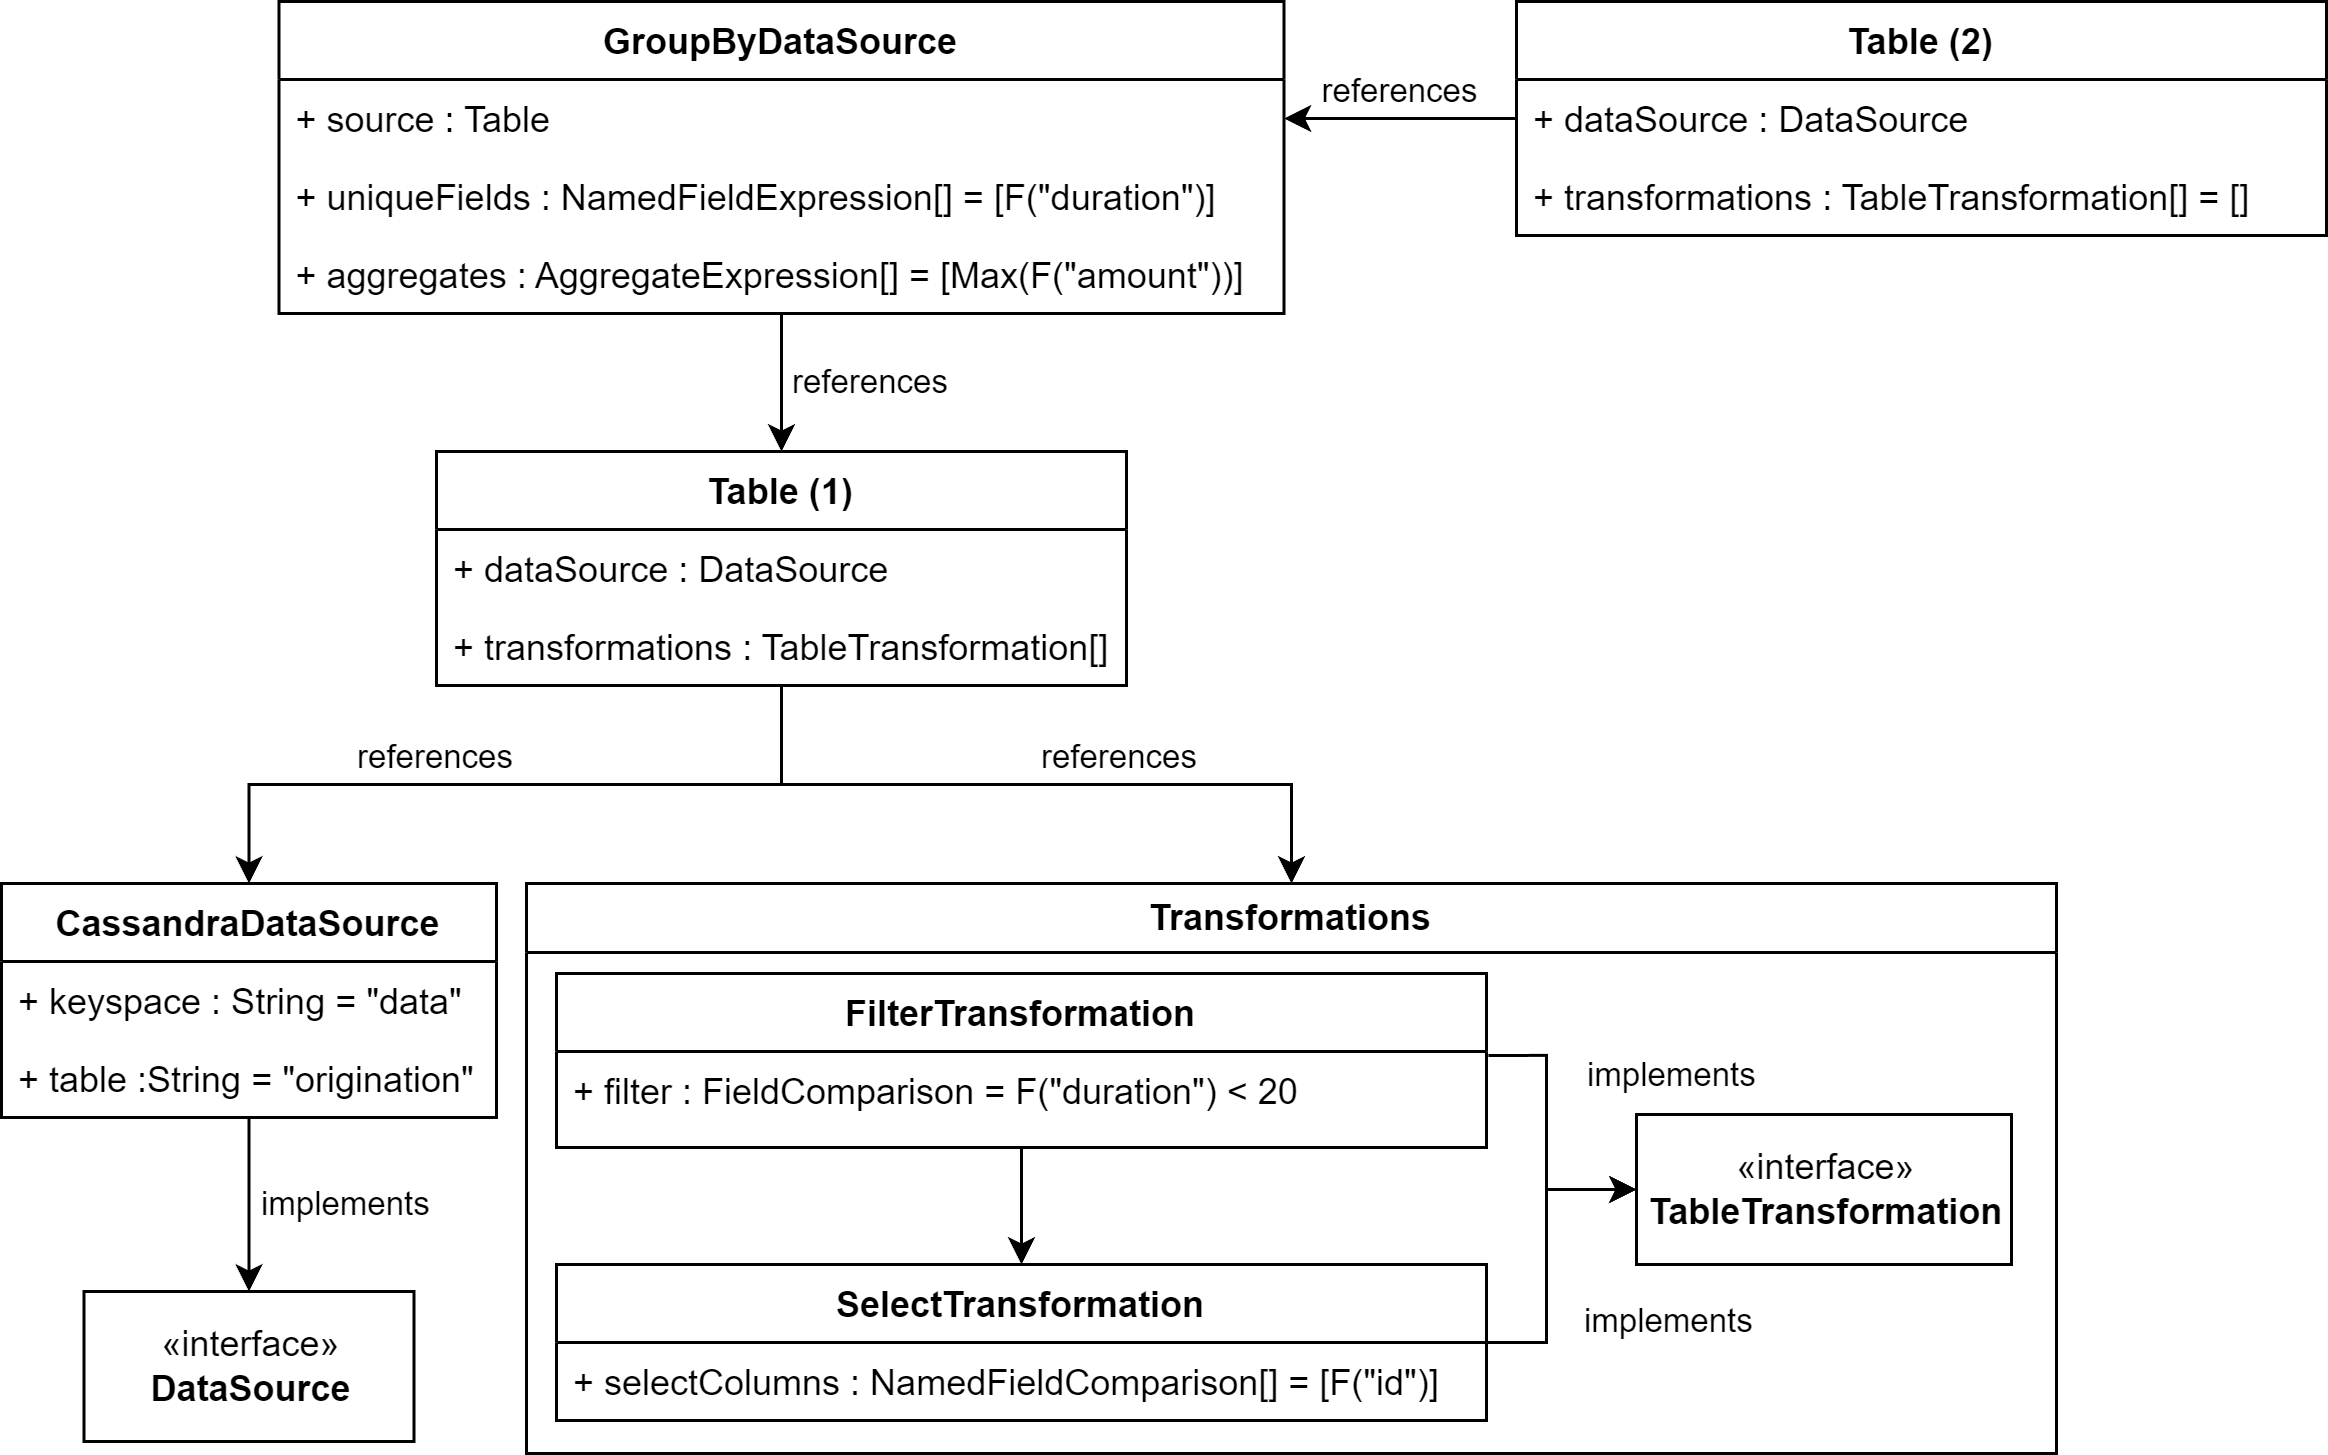
\includegraphics[width=0.75\textwidth]{chapters/diagrams/implementation/group-by-query}
	\linebreak
	\begin{python}
ClusterManager("orchestrator-service")
.cassandra_table("data", "origination")
.filter(F("duration") < 20)
.select(F("id"))
.group_by([F("duration")], [Max(F("amount"))])
.evaluate()
	\end{python}
	\caption{Example Group By Query}
	\label{fig:group-by-query}
\end{figure}

A \textit{Table} or \textit{DataSource} cannot be computed directly, but must first be split into partitions, which are provided by the \textit{DataSource}. These partitions are represented by the interface \textit{PartialDataSource}, with the partitioning method being specific to each implementation. The \textit{Table} class has a similar partial form, \textit{PartialTable}, which references a \textit{PartialDataSource} and can be computed directly. To demonstrate how to produce a final result from a set of partitions, Figure \ref{fig:partial-filter-select-query} shows a high-level example of one possible way of partitioning and computing the previous Filter and Select query.

\begin{figure}[htp]
	\centering
	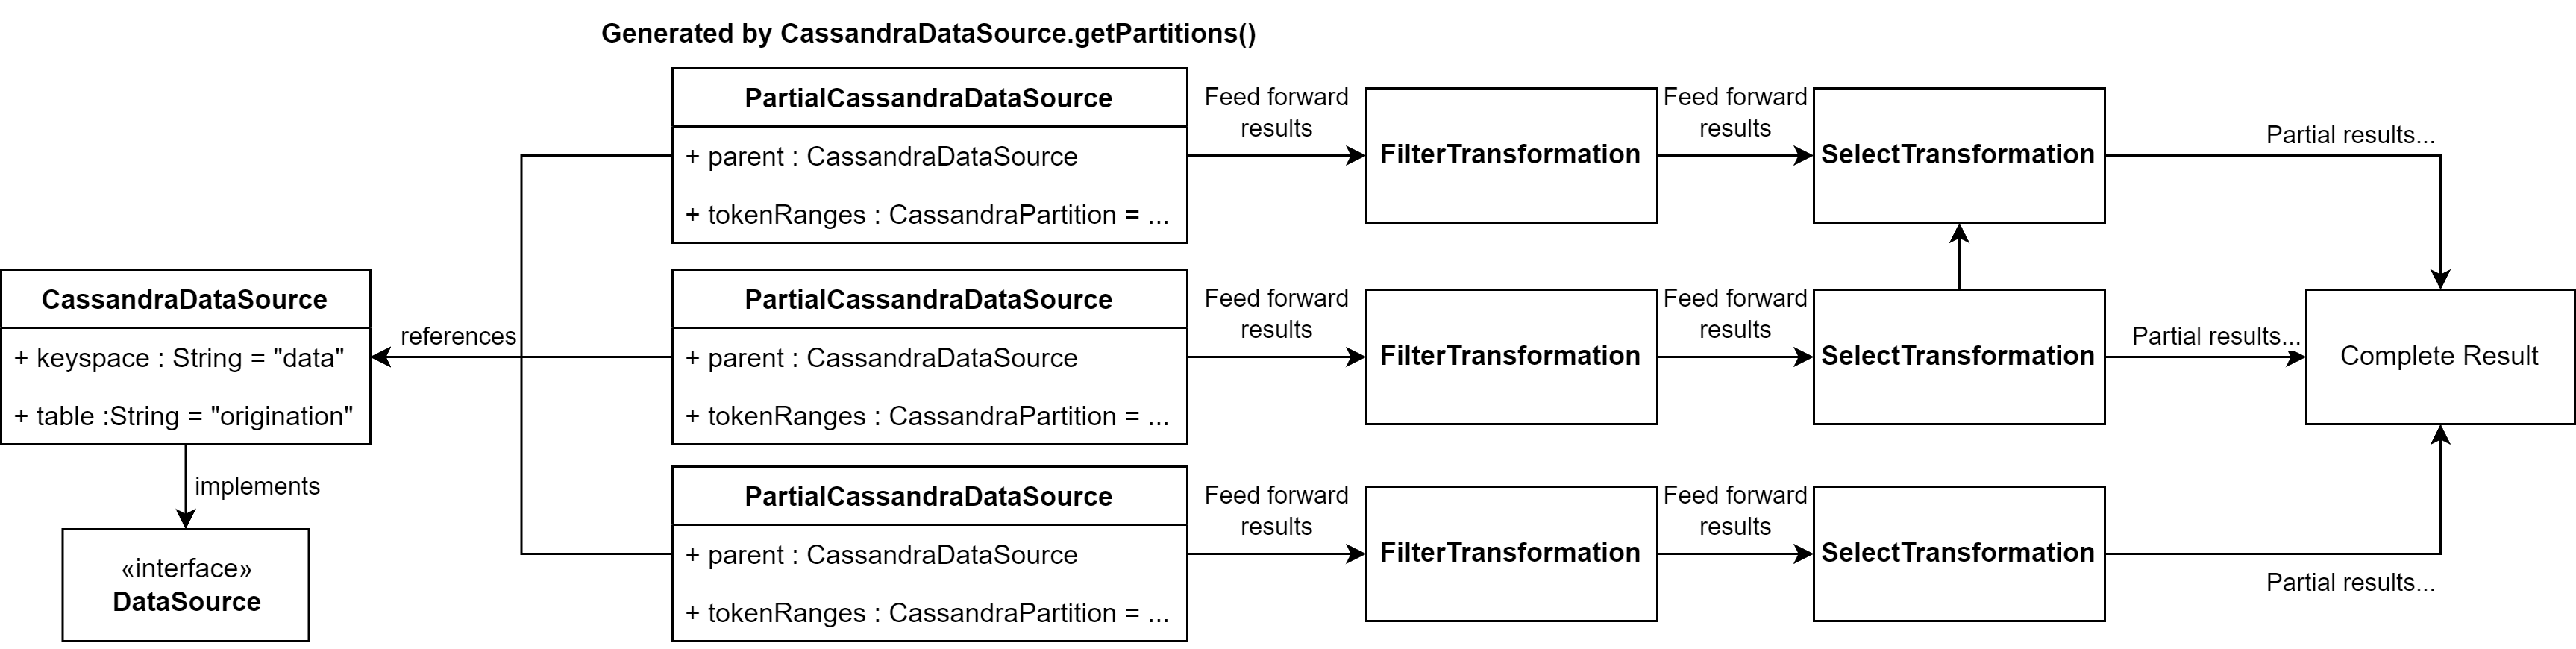
\includegraphics[width=\textwidth]{chapters/diagrams/implementation/partial-filter-select-query}
	\caption{Example Filter and Select Query}
	\label{fig:partial-filter-select-query}
\end{figure}


\pagebreak
\section{Data Store}
The data store allows the workers to store partially computed data, which can be reused in later parts of the query execution. In particular when workers are communicating with one another, it is likely that the data store will receive multiple simultaneous requests, presenting issues with handling concurrency and synchronisation.

The approach taken to solve this uses the actor model, first introduced in 1973 by Carl Hewitt \cite{hewitt1973session}. Specifically, the Akka Actors framework was chosen for a Scala actor model implementation \cite{akkaactors}. It abstracts away the complexity of synchronisation and thread management, modelling components of the system as actors. Each actor defines a set of accepted messages, and the response to each message. The framework then guarantees that an actor will only ever process one message at a time.

The data store is an actor which stores results as key-value pairs. Three kinds of data can be used as keys for storage: \textit{Table} computation results, \textit{DataSource} computation results and hashed data results, which are used when computing Group Bys. It uses a two-stage lookup, internally implemented using nested HashMaps. First, the full version of the data (\textit{Table} or \textit{DataSource}) is looked up, then the partial version (\textit{PartialTable} or \textit{PartialDataSource}). Partial forms always contain a reference to the full version, but not the other way around. Therefore, this design does not increase the insert time significantly, but it is particularly useful when reading or deleting a \textit{Table} or \textit{DataSource}. Otherwise, these operations would require searching the entire HashMap, turning the O(1) lookup time into O(n).

\subsection{Spill to Memory}
When operating on very large datasets, the dataset may be larger than the available memory of the workers. In this case, the JVM will run out of heap space, causing a crash when it tries to allocate more memory. Therefore, the data store has a module designed to move in-memory data onto disk to free up heap space, operating transparently from the perspective of other worker components. 

\paragraph{Storage Interface}
To implement the spill process, an interface, \textit{StoredTableResult}, is defined. This interface holds a key which corresponds to a result, and a \textit{get} operation to retrieve the result data. There are two subclasses with implementations: \textit{InMemoryTableResult} and \textit{ProtobufTableResult}. \textit{InMemoryTableResult} holds the result in-memory, and has a \textit{spillToDisk} method which moves the data to disk. \textit{ProtobufTableResult} holds a pointer to the data on-disk, reading the data from there when the \textit{get} operation is called.

\paragraph{Spill Process}
The data store is responsible for managing in-memory and on-disk data. Before almost every operation, it checks current memory utilisation, which is calculated using Java's \textit{Runtime} class \cite{javaruntimeclass}. If the utilisation is over a given threshold, the data store attempts to spill data to get below the threshold.

Figure \ref{fig:bytes-over-memory-threshold} shows how the number of bytes over a percentage threshold is calculated. The division calculates the current memory utilisation percentage, then the threshold is subtracted to get the percentage amount over the threshold. This is multiplied by the total number of bytes to get the result.

\begin{figure}[h]
	\centering
	\[ \left( \frac{\text{Bytes in Use}}{\text{Total Bytes Available}} - \text{Threshold} \right) * \text{Total Bytes Available} \]
	\caption{Number of Bytes Over Memory Threshold}
	\label{fig:bytes-over-memory-threshold}
\end{figure}

To perform the spill, the data store follows the decision tree shown in Figure \ref{fig:spill-to-disk-process}.

\begin{figure}[h]
	\centering
	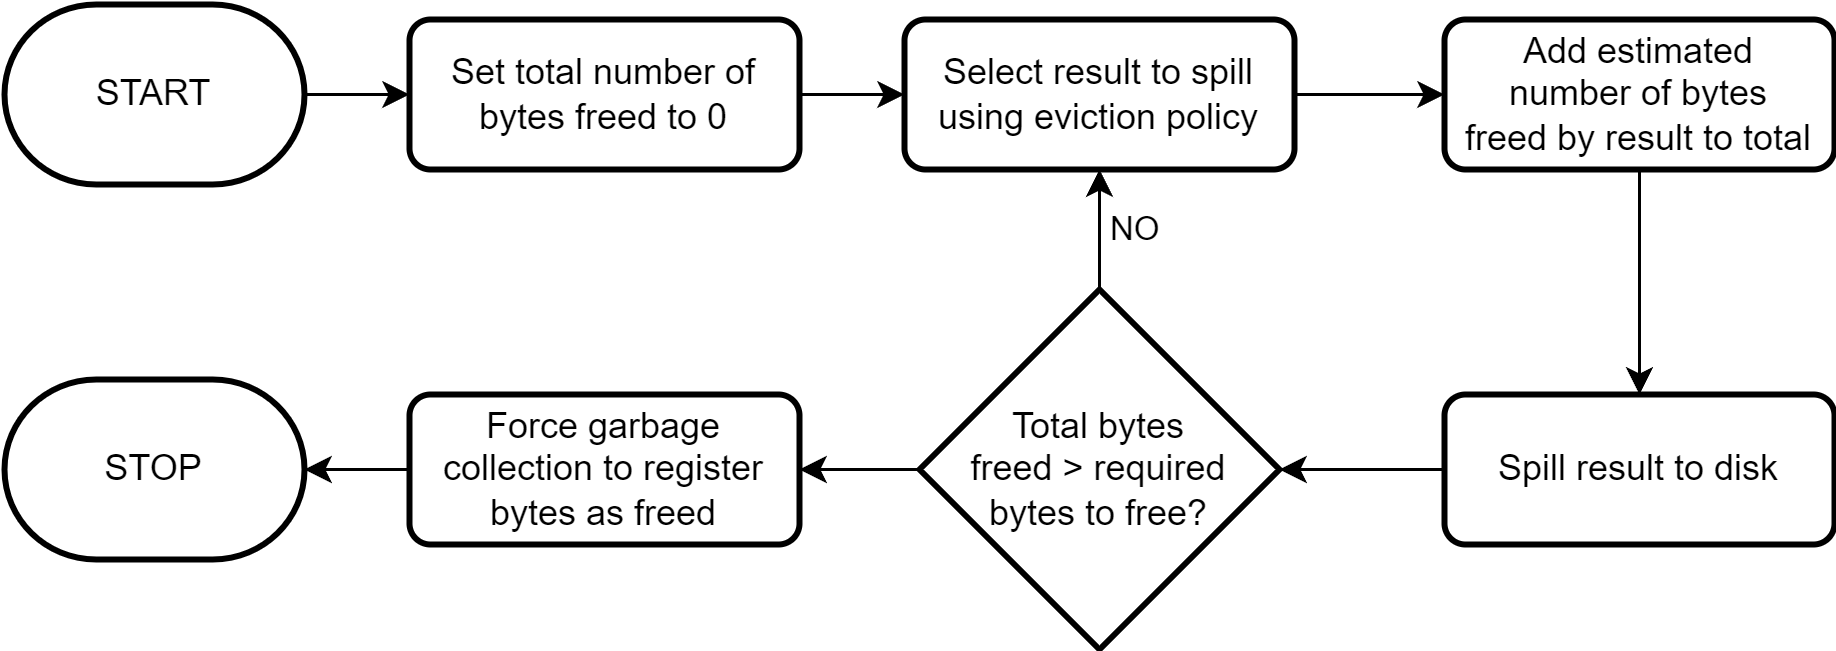
\includegraphics[width=0.6\textwidth]{chapters/diagrams/implementation/spill-to-disk-process}
	\caption{Spill to Disk Decision Tree}
	\label{fig:spill-to-disk-process}
\end{figure}

This process is not without flaws. It relies on no other classes in the current JVM instance holding references to any spilled results. In the controlled worker environment, this can be guaranteed, meaning the spill works reliably. 

\paragraph{Eviction Policy}
Finally, the policy for selecting spill results is important. A policy that does not fit the data store's usage could cause anti-patterns like the data store spilling a result, then immediately reading it back to memory. The data store uses a least-recently-used policy to select a result to spill, implemented using an ordered list.



\section{Partitioning}
One of the most important roles of the orchestrator during a computation is to calculate partitions. There are two situations where this is required:  pulling source data from Cassandra, and computing a Group By. The data model uses the \textit{DataSource} interface to represent computations that require new partitions. 

The goal of partitioning is to split a dataset into roughly equal chunks of a manageable size. Two things are required to do this: an estimate of the full size of a dataset, and a way of splitting the dataset to keep unique keys together. These are referred to as the partitioning requirements.

\subsection{Cassandra}\label{subsec:cassandra}
Cassandra was selected for persistent storage because its features meet the partitioning requirements. As discussed in Section \ref{subsec:cassandra-design}, Cassandra's token range system natively provides a way of splitting the source dataset. Furthermore, Cassandra provides size estimates for any table automatically in the \texttt{system.size\char`_estimates} table.

%Cassandra was selected for persistent storage because the distributed storage model matches the type of partitioning the system requires. When generating new partitions, The Cassandra \textit{DataSource} investigates the source data in the database, and generates an appropriate number of partitions. This process is described below.

A table size estimate can be used to derive a token range size estimate using the equation in Figure \ref{fig:token-range-estimation}. The division calculates the percentage of the full token range that the given token range represents.

\begin{figure}[h]
	\centering
	\[ \frac{\text{Number of Tokens in Token Range}}{\text{Total Number of Tokens: } ((2^{63}-1) - (-2^{63}))} \times \text{Estimated Table Size} \]
	\caption{Token Range Size Estimation Equation}
	\label{fig:token-range-estimation}
\end{figure}

\pagebreak
Using this equation, the token ranges which each node is responsible for storing are collected. Then, the orchestrator performs a joining and splitting process over each node, depending on the size of the token ranges. The set of token ranges produced by this process are the partitions used during the computation. Figure \ref{fig:cassandra-partitioning-decision-tree} shows the full process for generating the output partitions.

\begin{figure}[h]
	\centering
	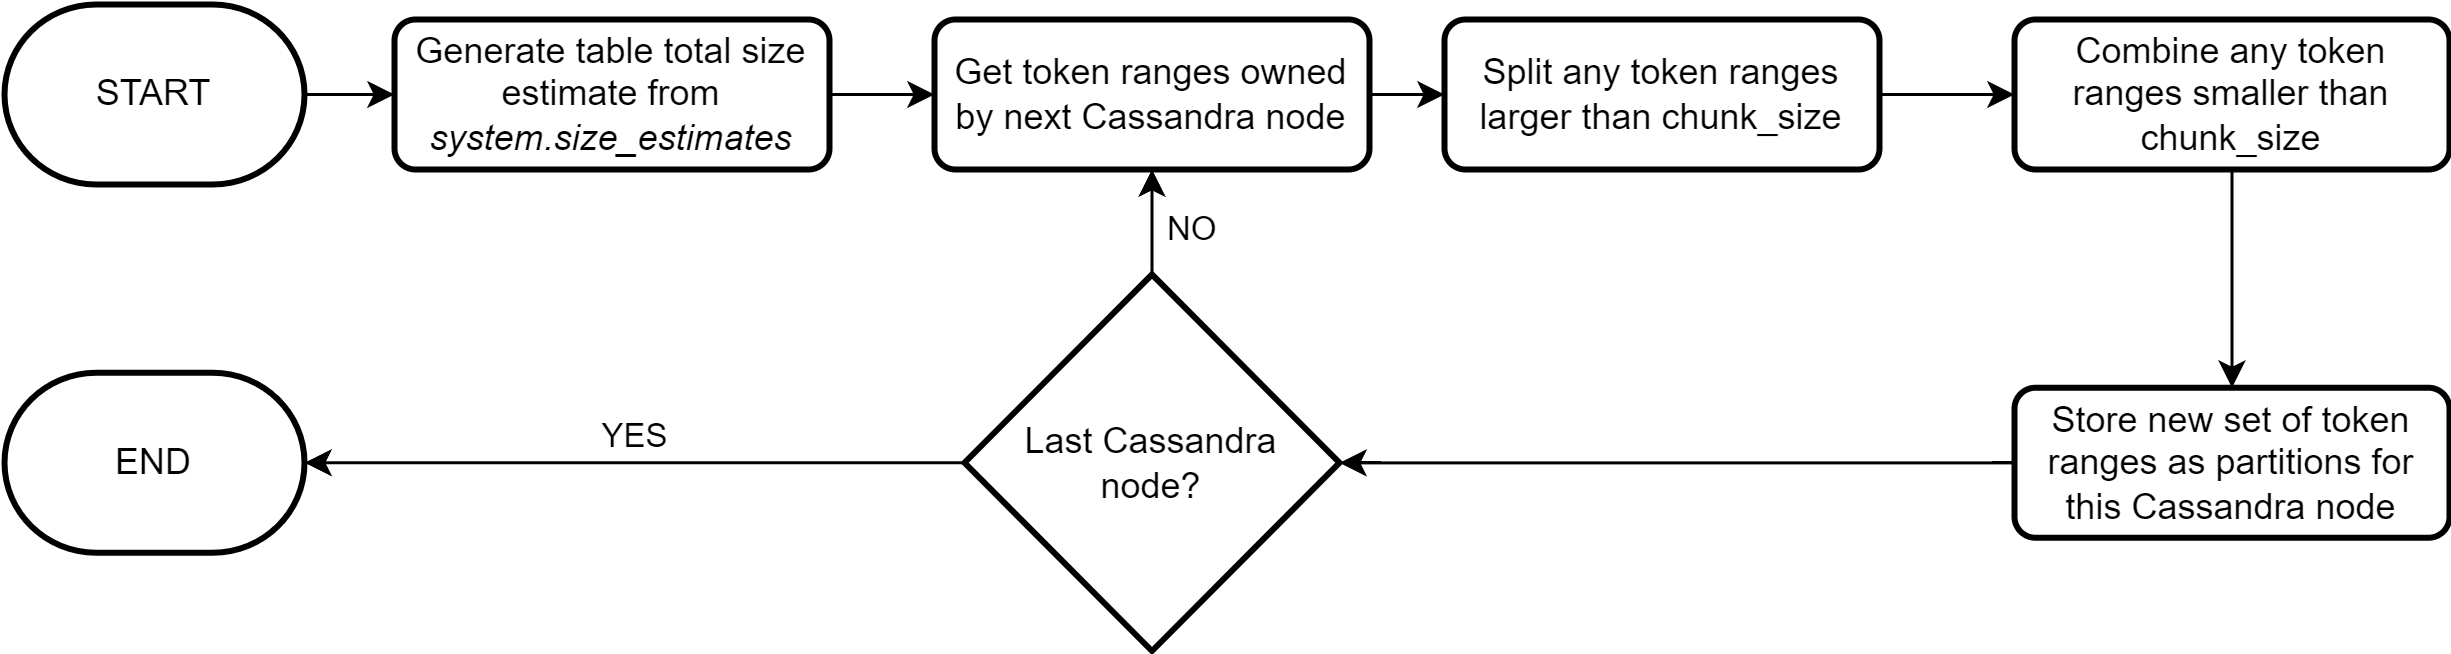
\includegraphics[width=0.8\textwidth]{chapters/diagrams/implementation/cassandra-partitioning-decision-tree}
	\caption{Cassandra Partitioning Process}
	\label{fig:cassandra-partitioning-decision-tree}
\end{figure}


Figure \ref{fig:cassandra-split-process} demonstrates the token splitting process. The system calculates how many times larger the token range is than the goal partition size, then splits the token range evenly by that amount.

\begin{figure}[h]
	\centering
	\subfloat[\centering Equation]{\raisebox{1.5cm}{$ \text{Number of Splits} = \frac{\text{Token Range Size}}{\text{Chunk Size}} $}}
	\qquad
	\subfloat[\centering Example]{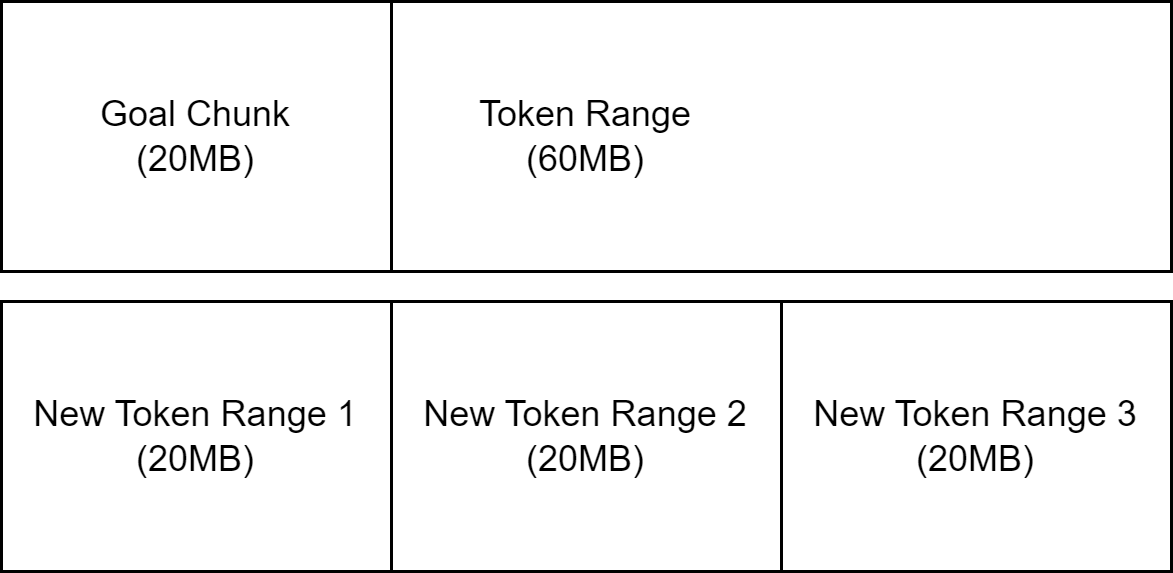
\includegraphics[width=0.4\textwidth]{chapters/diagrams/implementation/cassandra-split-example}}
	\caption{Token Range Splitting}
	\label{fig:cassandra-split-process}
\end{figure}

Figure \ref{fig:cassandra-join-process} provides an example of the joining process. Given a list of token ranges, the orchestrator combines sequential elements until they are larger than the goal partition size, then it marks this as a new partition. The list is sorted by size ascending to combine small token ranges together, producing fewer partitions.

\begin{figure}[h]
	\centering
	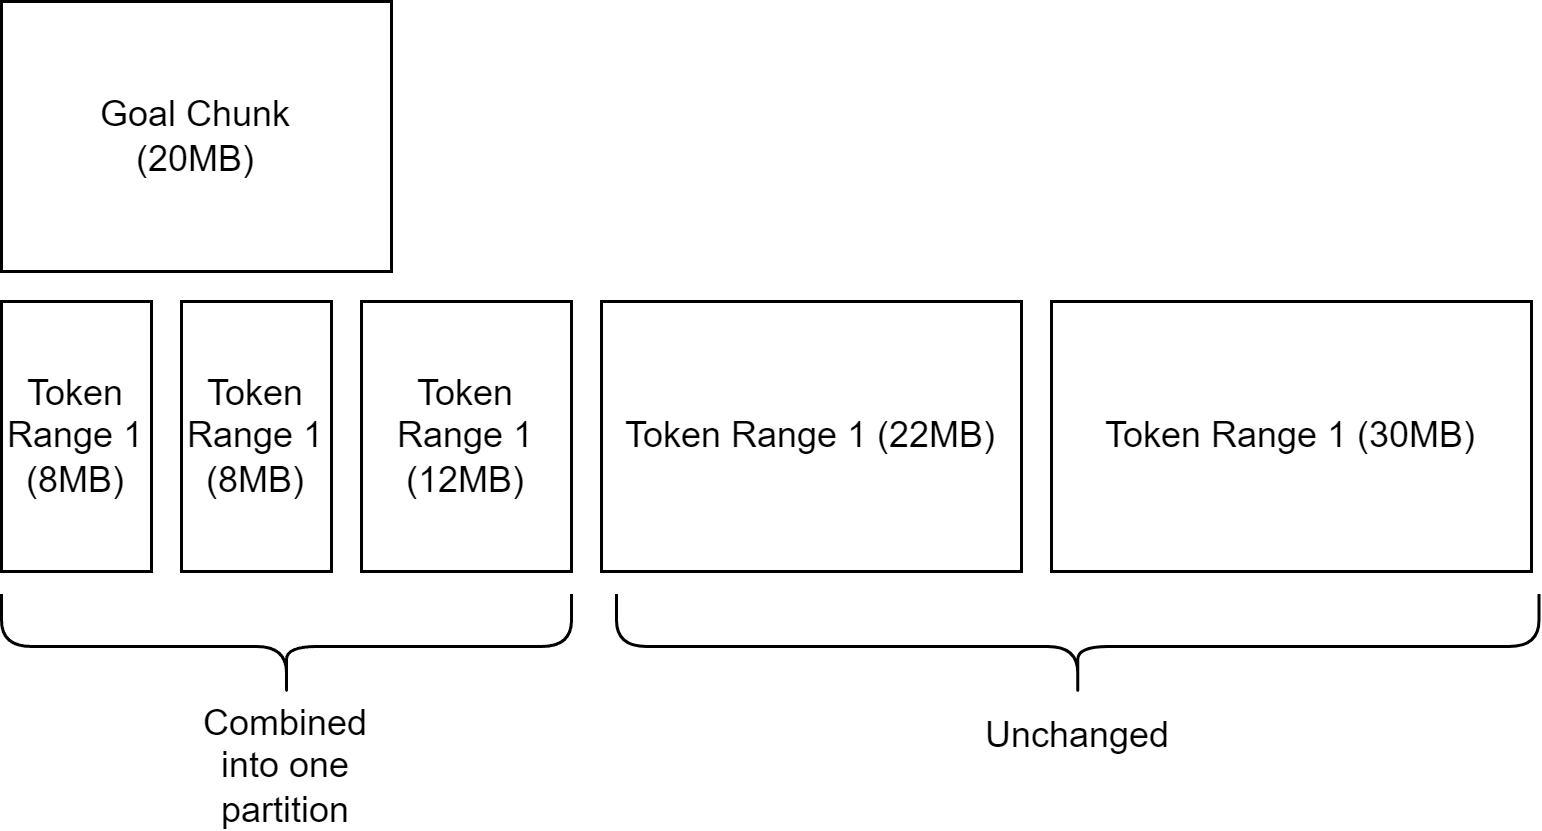
\includegraphics[width=0.5\textwidth]{chapters/diagrams/implementation/cassandra-join-example}
	\caption{Token Range Joining Example}
	\label{fig:cassandra-join-process}
\end{figure}

%The Cassandra Java Driver provides helper functions to perform the joining and splitting of token ranges; the system simply calculates how much joining or splitting is required. % doesn't really add anything

\pagebreak
\subsection{Cassandra Data Co-Location}\label{subsec:colocation}
From a list of partitions for each Cassandra node, the system attempts to co-locate workers to Cassandra nodes. The goal of this process is to produce an \textit{optimal assignment}, where each partition is matched to one or more workers to minimise network latency when importing data from Cassandra.

To do this, each worker first calculates its closest Cassandra node by opening a TCP connection with each Cassandra node, averaging the latency over multiple attempts, and selecting the node with the lowest latency. The orchestrator uses this information to match each worker to a Cassandra node and its corresponding list of partitions, producing an optimal assignment between workers and partitions. Partitions can have no co-located worker nodes. In this case, the partitions are unassigned, and the work assignment algorithm handles their allocation; see Section \ref{subsec:get-partition} for details. Figure \ref{fig:optimal-assignment-example} shows an example cluster with three physical nodes, and the corresponding optimal assignment.

\begin{figure}[h]
	\centering
	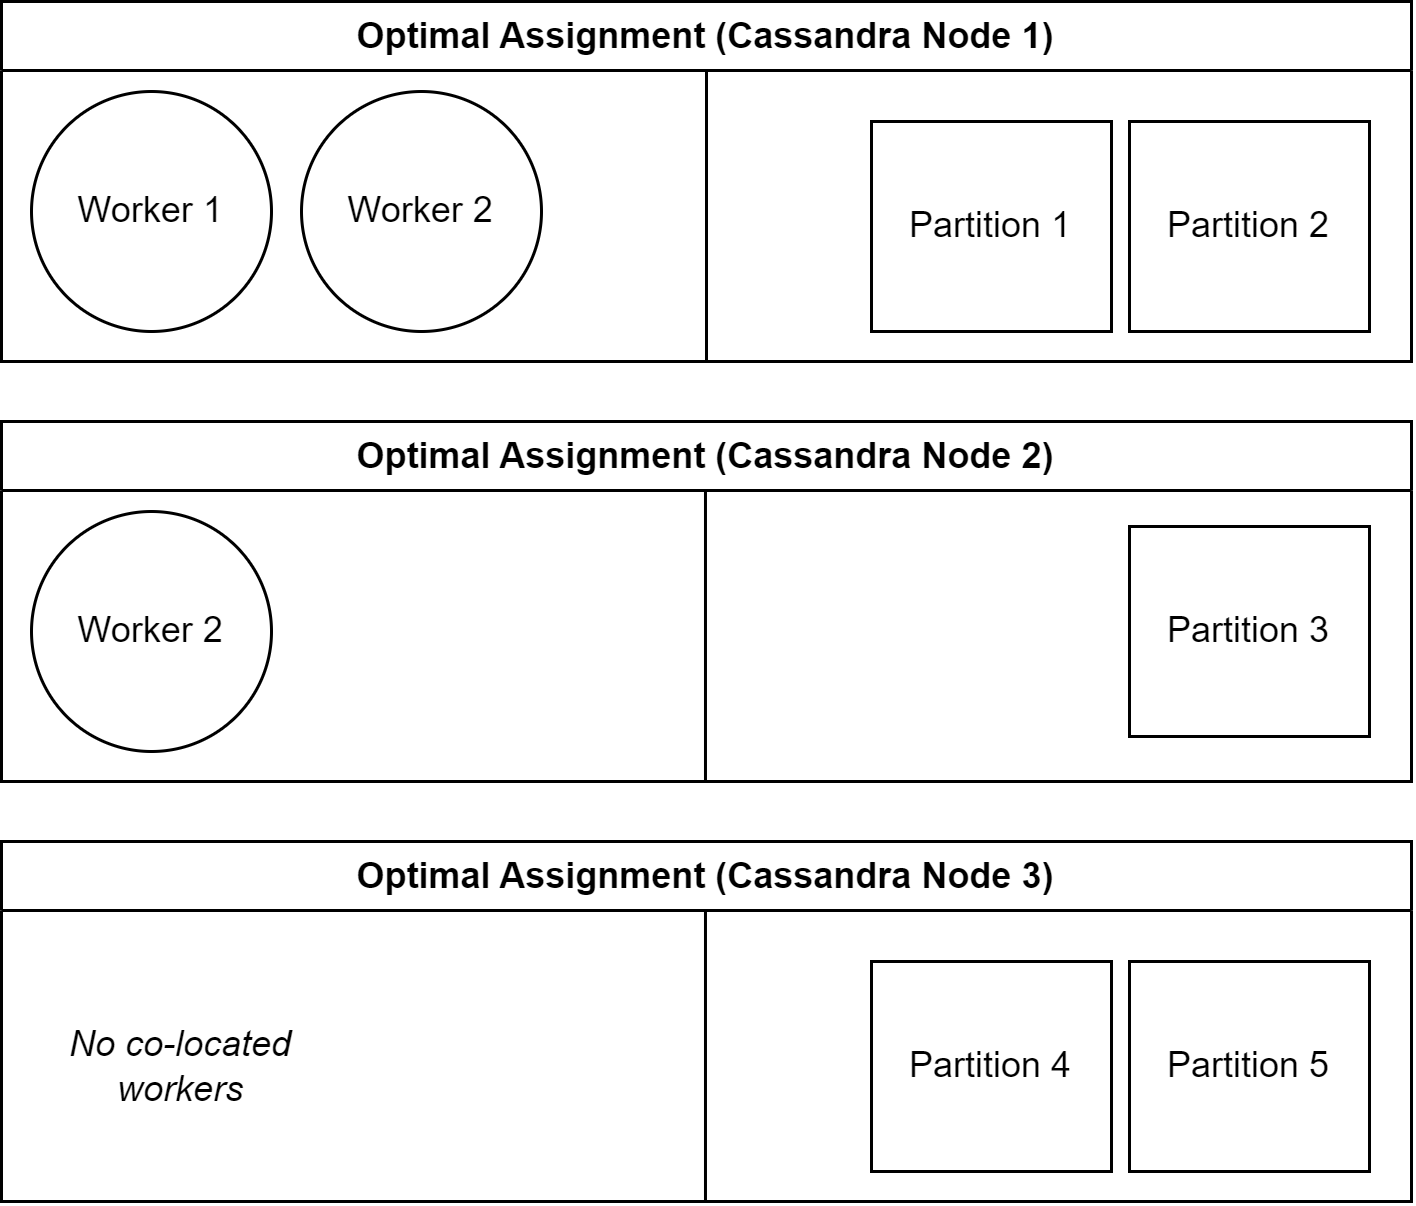
\includegraphics[width=0.8\textwidth]{chapters/diagrams/implementation/optimal-assignment-example}
	\caption{Optimal Assignment Example}
	\label{fig:optimal-assignment-example}
\end{figure}

\subsection{Group By}\label{subsec:group-by}
The Group By operation takes any number of \textit{NamedFieldExpressions} as unique keys, and any number of \textit{AggregateExpressions} to calculate for each combination of unique keys. This operation is not reliant on external components, so custom implementations must be used to meet the partitioning requirements.

The process of calculating a Group By is described below. These steps are controlled by the orchestrator during the execution of \textit{GetPartition}; see Section \ref{subsec:get-partition} for details.

\paragraph{Partitions}
The first step is to compute the number of output partitions for the Group By, which is based on a size estimate of the dependent \textit{Table}. To generate this, a class from Apache Spark was reused, with some changes for compatibility with Scala 3 \cite{zaharia2016spark}. This class provides a static method \textit{estimate} which produces a size estimate, in bytes, for any Scala object. The orchestrator calls this on all partial results across all workers, and the estimates are totalled to calculate the total size of all data for a \textit{Table}. Figure \ref{fig:group-by-num-partitions} shows how the size estimate can be used to derive the total number of partitions to generate for a \textit{Table}.

\begin{figure}[h]
	\centering
	\[ \frac{\text{Table Size Estimate}}{\text{Goal Partition Size}} \]
	\caption{Group By - Total Partitions}
	\label{fig:group-by-num-partitions}
\end{figure}


\pagebreak
\paragraph{Hashing} 
A unique partition is defined as a tuple, shown in Figure \ref{fig:group-by-unique-partition}. Hashing, combined with the modulo operation, is used to assign rows of data to partitions. In particular, Murmur3Hash is used as the hashing algorithm, used in Cassandra and provided natively by Scala \cite{murmur3hash}. Figure \ref{fig:group-by-partition-assign} shows the high-level equation for assigning rows to partitions. This equation maps all rows with the same combination of unique keys to the same partition.

\begin{figure}[h]
	\centering
	\[ (\text{Total Number of Partitions}, \text{Assigned Partition Number}) \]
	\caption{Group By - Unique Partition Definition}
	\label{fig:group-by-unique-partition}
\end{figure} 

\begin{figure}[h]
	\centering
	\[ \text{Assigned Partition Number} \; = \; Murmur3Hash(\text{Unique Key Data}) \; \%  \; \text{Total Number of Partitions} \]
	\caption{Group By - Row Partition Assignment}
	\label{fig:group-by-partition-assign}
\end{figure} 

\paragraph{Computation}
After the hashes are computed and a worker is assigned a particular partition, it must cross-communicate with all other workers to fetch any data relating to that partition to ensure that the partition data is complete. To do this, the worker makes requests to all other workers, and they stream the header and rows of their partial data back. When a Group By is being computed, a worker will likely be simultaneously receiving data from another worker, and sending a different set of data to it. This makes the actor system driving the data store in each worker particularly valuable, as it provides thread-safe concurrent access to the data store.

Once a worker has collected all partition data, the groups are computed using a built-in Scala operation, and the \textit{AggregateExpressions} are evaluated for each group.

\paragraph{Deletion}
The last step of computing a Group By is to remove the hashed partition data stored on each worker, which is handled by the orchestrator automatically.



\section{Row-Level Computations}
Once partitions have been delegated to the workers, performing the computation is straightforward. 

\subsection{Select}\label{subsec:select-computation}
This operation takes any number of \textit{NamedFieldExpressions}. To compute a result, each \textit{NamedFieldExpression} is mapped over each input result row. 

\subsection{Filter}\label{subsec:filter-computation}
This operation takes a \textit{FieldComparison}, or a combined comparison. To compute, the comparison is mapped over each input result row, removing any rows where the comparison returns \texttt{false}.



\section{Query Plan}
Query Plans are the process through which the orchestrator can compute a user-defined query, to get a result. They are a sequence of \textit{QueryPlanItems}, which define a single step. Each \textit{QueryPlanItem} has an \textit{execute} method, which will make some change to the state of all workers in the cluster when called. Both \textit{DataSource} and \textit{Table} have a function that generates the full Query Plan to compute their output, and a second Query Plan to clear the data store of their output. 

Figure \ref{fig:filter-group-by-query-plan} shows the query plans for the Filter and Select query (Section \ref{fig:filter-select-query}) and Group By Query (Section \ref{fig:group-by-query}).

\begin{figure}[h]
	\centering
	\subfloat[\centering Filter and Select Query]{{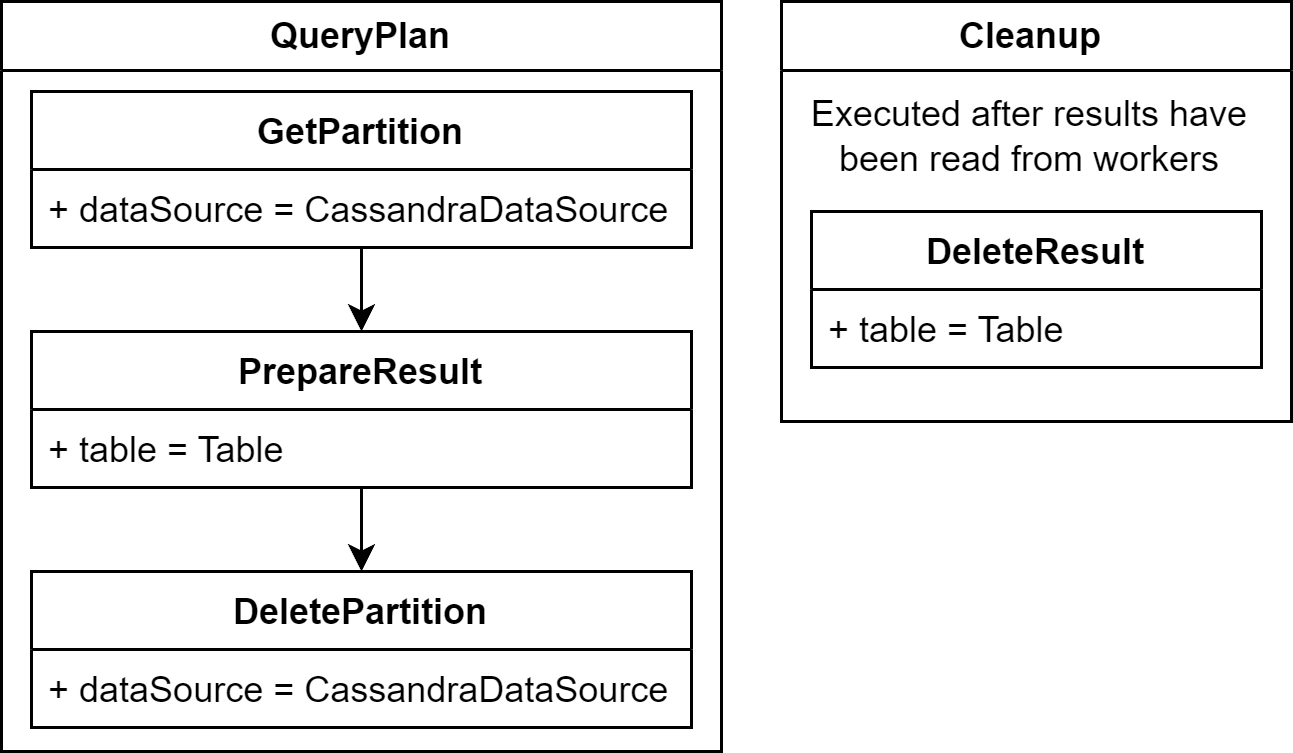
\includegraphics[width=0.35\textwidth]{chapters/diagrams/implementation/filter-select-query-plan}}}
	\qquad
	\subfloat[\centering Group By Query]{{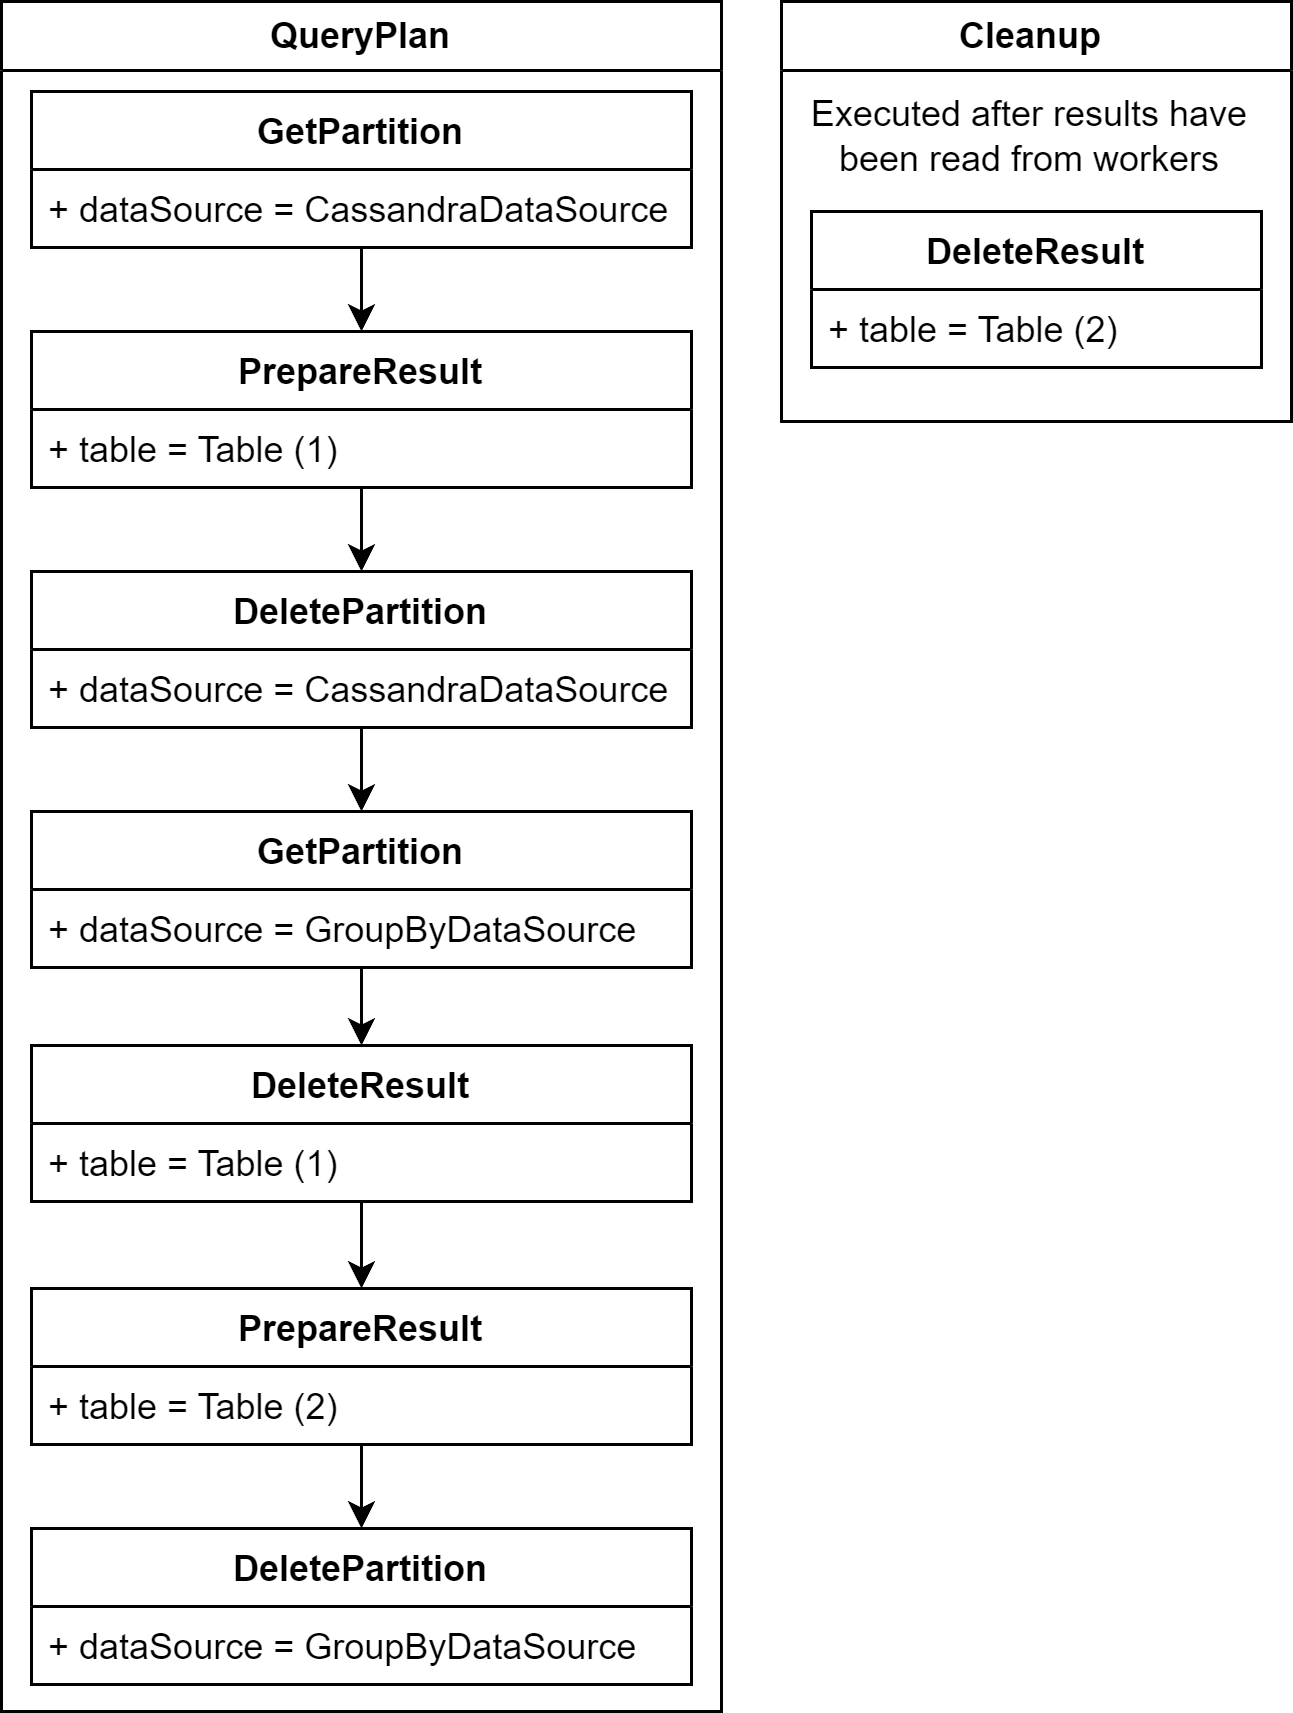
\includegraphics[width=0.35\textwidth]{chapters/diagrams/implementation/group-by-query-plan}}}
	\caption{Query Plans - Filter-Select and Group By Query}%
	\label{fig:filter-group-by-query-plan}
\end{figure}

\subsection{GetPartition}\label{subsec:get-partition}
This is the most complex \textit{QueryPlanItem}, encapsulating a number of steps in order to compute and store the partitions of a \textit{DataSource}. There are two main flows depending on if the \textit{DataSource} has dependent Tables.

If the \textit{DataSource} has no dependencies, for example when pulling data from Cassandra, then Figure \ref{fig:get-partition-no-dependencies} shows the process for this item. 

\begin{figure}[h]
	\centering
	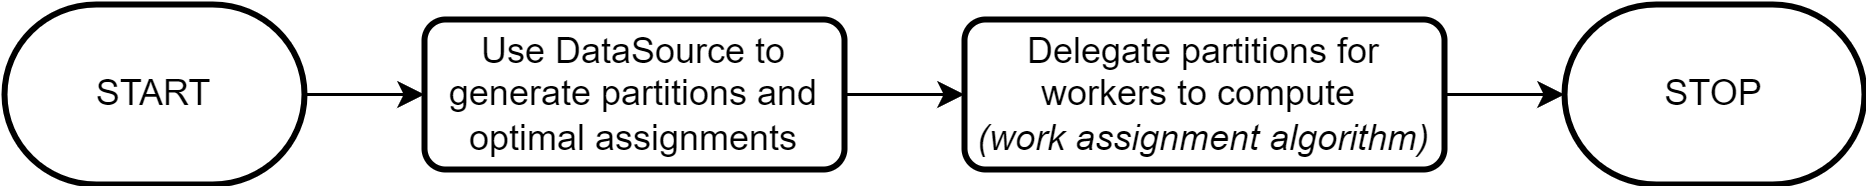
\includegraphics[width=0.8\textwidth]{chapters/diagrams/implementation/get-partition-no-dependencies-flow}
	\caption{Get Partition Execution - Without Dependencies}
	\label{fig:get-partition-no-dependencies}
\end{figure}

\pagebreak
If the \textit{DataSource} has dependencies, then Figure \ref{fig:get-partition-dependencies} shows the process for this item. These steps are the same as when calculating a Group By (Section \ref{subsec:group-by}). First, the partitions and optimal assignments are generated, then the dependency data is hashed based on the number of partitions to generate. Both of these steps are implementation-specific, and are therefore abstracted behind the \textit{DataSource} interface. 

The work assignment algorithm is then run to delegate partitions to the workers, followed by deleting the hashed dependency data. These steps do not change based on the \textit{DataSource}, so are handled exclusively by \textit{GetPartition}.
\begin{figure}[h]
	\centering
	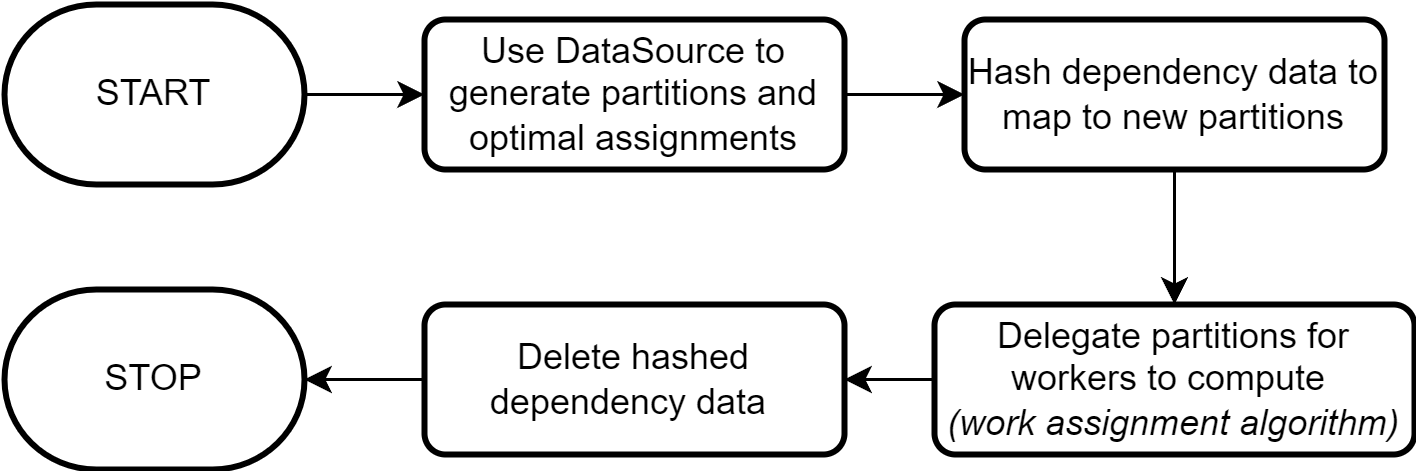
\includegraphics[width=0.7\textwidth]{chapters/diagrams/implementation/get-partition-dependencies-flow}
	\caption{Get Partition Execution - With Dependencies}
	\label{fig:get-partition-dependencies}
\end{figure}

\paragraph{Work Assignment Algorithm} % can probably cut some here
\textit{GetPartition} manages the process of delegating partitions to workers for computation using the Work Assignment Algorithm. A simple solution would use a round-robin process to match optimal assignments to their co-located workers, delegating work when a request finishes and stopping when the assignments are empty. However, this can result in idle workers, for example if one worker's list of optimal assignments is shorter than the others, or if one worker is unexpectedly slow.

Ideally, workers would compute all of their own optimal partitions first, then compute the partitions that were originally assigned to other workers. This implements dynamic load balancing: a faster-running worker can take on proportionally more requests, and no worker will be idle unless all partitions are computed. However, race conditions need to be avoided, like delegating same partition twice to different workers.

The actor model is ideal for this situation \cite{hewitt1973session}. Sets of optimal partitions are modelled as \textit{producer} actors, and the workers as \textit{consumers}. Producers respond to requests for work with partitions to be computed. Consumers are given an ordered list of producers, then repeatedly request and compute work from each in order. Each consumer has the producer holding that consumer's optimal partitions first in the list. A counter actor tracks the number of completed partitions, sending a signal when all partitions have been computed, or an error if any worker fails.

This solution also handles unassigned partitions with no co-located workers; this producer is placed last in the list of producers for each consumer, where they will eventually be processed.

Figure \ref{fig:producer-consumer-model-example} provides the initial state of this model, using the example optimal assignment from Figure \ref{fig:optimal-assignment-example}. Dark arrows represent the producer which the consumer will empty first, containing its optimal assignments, and light grey arrows represent other producers which the consumer can access. Producer 3 is not first for any worker, but will eventually be checked by the workers when all others are exhausted.

\begin{figure}[h]
	\centering
	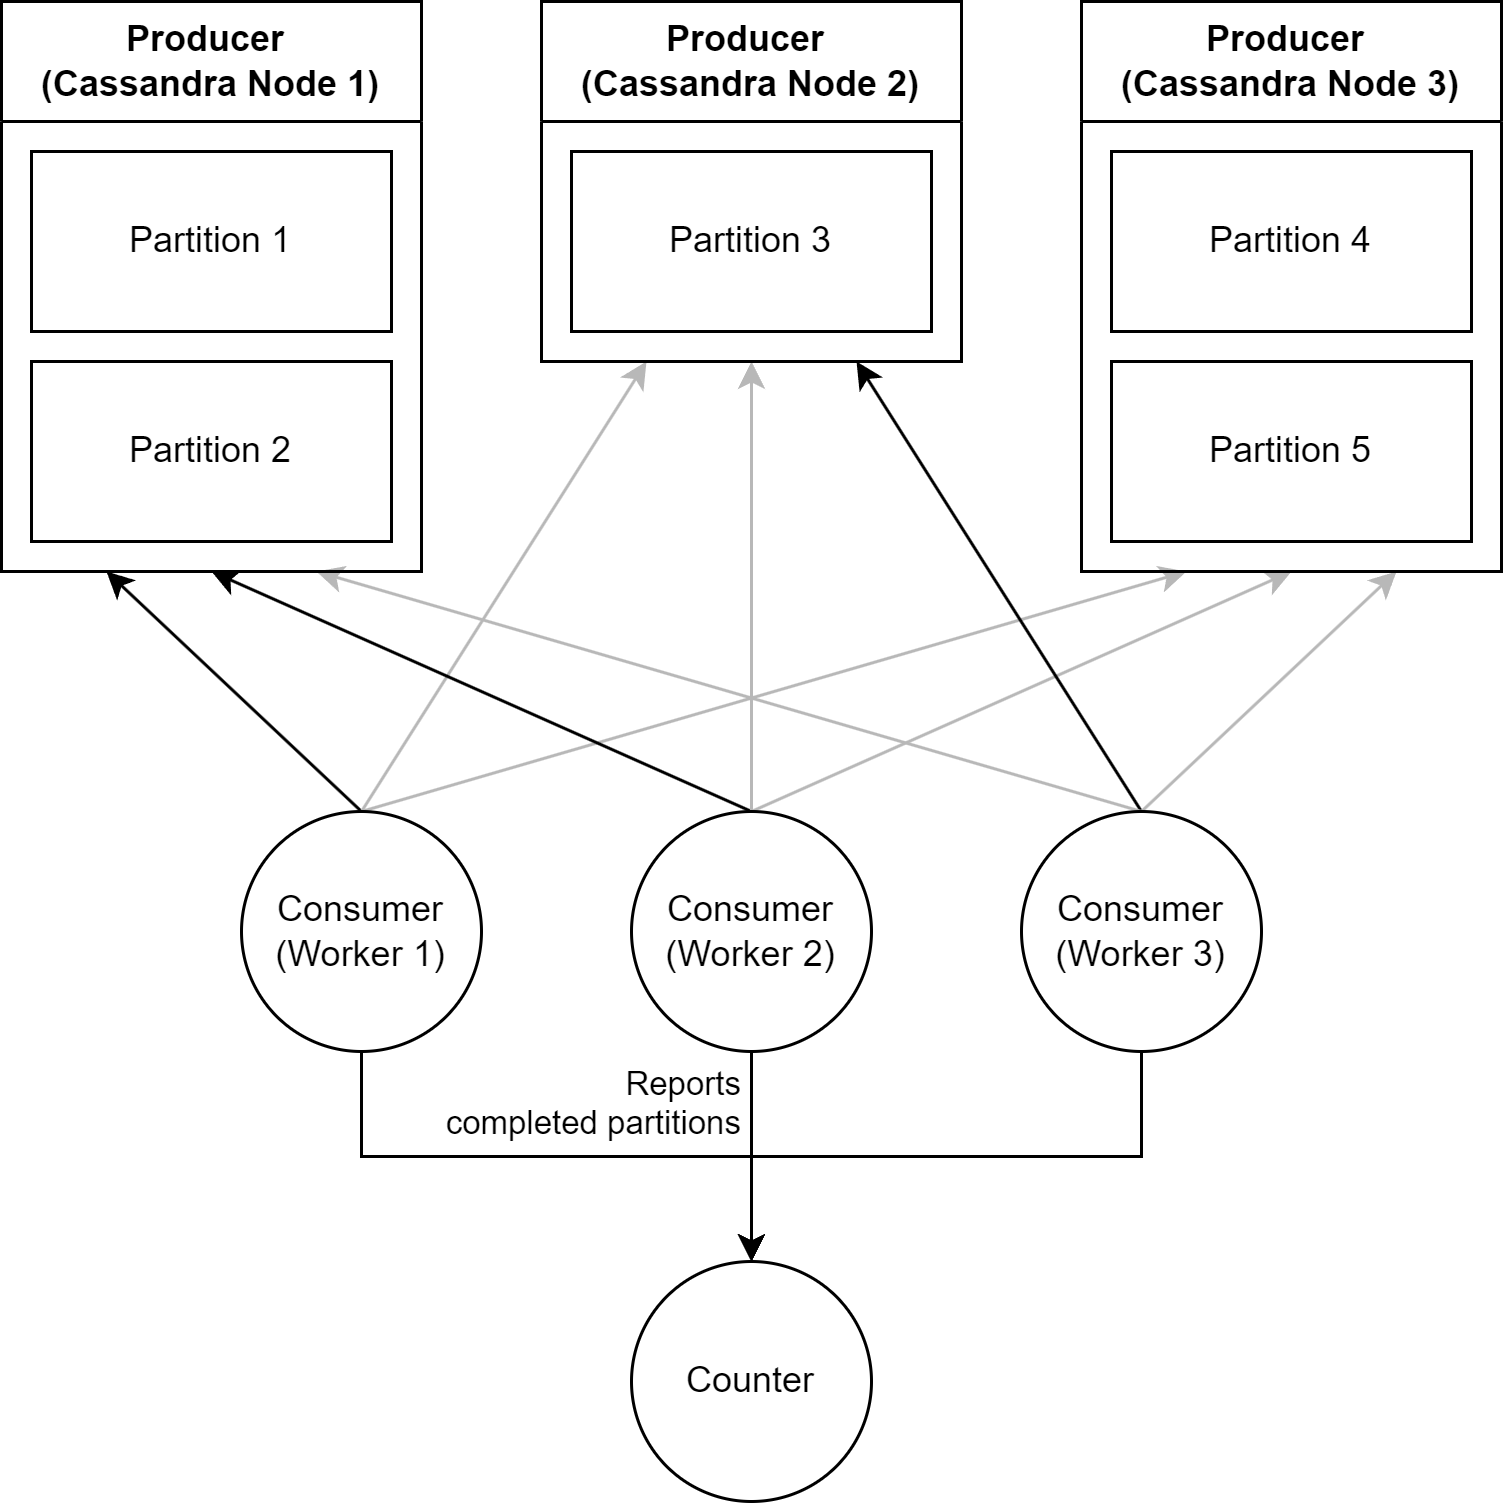
\includegraphics[width=0.5\textwidth]{chapters/diagrams/implementation/producer-consumer-model-example}
	\caption{Producer Consumer Model Example}
	\label{fig:producer-consumer-model-example}
\end{figure}

\pagebreak
\subsection{PrepareResult}
This \textit{QueryPlanItem} computes a \textit{Table} from the partitions of a \textit{DataSource} that are already stored on the workers. Therefore, it will always be called after \textit{GetPartition}, with the new partitions as an argument. A modified version of \textit{GetPartition}'s actor system is used to iterate through all partitions on each worker, sending a request to perform the \textit{Table} computation for each.

\subsection{DeleteResult and DeletePartition}
\textit{DeletePartition} and \textit{DeleteResult} are \textit{QueryPlanItems} for removing the results of a \textit{GetPartition} and \textit{PrepareResult} operation, respectively. They send a single request to each worker, which will remove all results that relate to a \textit{Table} or \textit{DataSource}, and respond with a confirmation.

\subsection{Result Collation}
After all the steps of a query are completed, the final results are stored across all the workers. The orchestrator makes a request to all workers to return the computed results, and each worker iterates over all partial results in the data store, streaming the data back to the orchestrator. An actor system pipes the concurrent responses into a single thread, which combines the results and streams them to the frontend. The request is initiated by the orchestrator because gRPC requires that one system act as a server, and another as a client. For the query plan model, it makes most sense for the workers to be servers, so this model is also used for result collation.

\pagebreak
\section{Deployment}
As discussed in Chapter \ref{cha:design}, Kubernetes was chosen to manage all nodes in the cluster. One feature that makes it useful for the system is scheduling rules, which provide Kubernetes with information about how containers should be assigned to physical nodes.

As previously described in Section \ref{subsec:colocation}, workers determine their closest Cassandra node automatically based on latency. To make the best use of the cluster, workers should be distributed evenly across all nodes that have a Cassandra node. This is implemented by these scheduling rules:
\begin{enumerate}
	\item If possible, workers should be placed on the same Kubernetes node as a Cassandra node.
	\item Workers should not be placed on the same node as other workers.
\end{enumerate}

The scheduling rules are preferences rather than requirements, meaning Kubernetes is still able to schedule the nodes if there are more workers than Cassandra nodes.

\subsection{CI/CD}
To aid in deploying to Kubernetes, continuous integration/continuous deployment (CI/CD) pipelines are used for each major system component, specifically using GitHub Actions \cite{githubactions}. Each pipeline runs all unit tests for the component, and provided they succeed, builds a docker container and pushes it to a container registry, ready for use in the Kubernetes cluster.

